\documentclass[
  reprint,
  amsmath,
  amssymb,
  aps,
  pra,
  nofootinbib,
  superscriptaddress,
  floatfix
]{revtex4-2}

\usepackage[T1]{fontenc}
\usepackage{lmodern}
\usepackage{graphicx}
\usepackage{booktabs}
\usepackage{bm}
\usepackage{mathtools}
\usepackage{xcolor}
\usepackage{hyperref}

\newcommand{\placeholder}[1]{\textcolor{red!70!black}{\ifmmode\left[#1\right]\else\textsf{[#1]}\fi}}
\newcommand{\tentative}[1]{\textcolor{red!70!black}{#1}}
\newcommand{\structlabel}[1]{\noindent\mbox{\tentative{#1.}}~}

\newcommand{\Oset}{\mathcal{O}}
\newcommand{\Gset}{\mathcal{G}}
\newcommand{\Rset}{\mathcal{R}}
\newcommand{\Sset}{\mathcal{S}}
\newcommand{\Hcal}{\mathcal{H}}
\newcommand{\Bcal}{\mathcal{B}}
\newcommand{\Ocal}{\mathcal{O}}
\newcommand{\Ecal}{\mathcal{E}}
\newcommand{\Acal}{\mathcal{A}}
\newcommand{\Scal}{\mathcal{S}}
\newcommand{\Ncal}{\mathcal{N}}
\newcommand{\Gcal}{\mathcal{G}}
\newcommand{\Fcal}{\mathcal{F}}
\newcommand{\Ccal}{\mathcal{C}}
\newcommand{\Qcal}{\mathcal{Q}}
\newcommand{\Vcal}{\mathcal{V}}
\newcommand{\Mcal}{\mathcal{M}}
\newcommand{\Wcal}{\mathcal{W}}
\newcommand{\Dcal}{\mathcal{D}}
\newcommand{\Pcal}{\mathcal{P}}
\newcommand{\Tcal}{\mathcal{T}}
\newcommand{\Ucal}{\mathcal{U}}
\newcommand{\dd}{\mathrm{d}}
\newcommand{\ii}{\mathrm{i}}
\newcommand{\ee}{\mathrm{e}}
\newcommand{\TR}{\mathrm{TR}}
\newcommand{\ex}{\mathrm{ex}}
\newcommand{\ctrl}{\mathrm{ctrl}}
\newcommand{\stat}{\mathrm{stat}}
\newcommand{\dyn}{\mathrm{dyn}}
\newcommand{\drv}{\mathrm{drv}}
\newcommand{\obs}{\mathrm{obs}}
\newcommand{\stay}{\mathrm{stay}}
\newcommand{\app}{\mathrm{append}}
\newcommand{\ablate}{\mathrm{ablate}}
\newcommand{\qse}{\mathrm{QSE}}
\newcommand{\eqse}{\mathrm{eQSE}}
\newcommand{\ed}{\mathrm{ED}}
\newcommand{\lf}{\mathrm{LF}}
\newcommand{\fb}{\mathrm{fb}}
\newcommand{\fs}{\mathrm{f}}
\newcommand{\bs}{\mathrm{b}}
\newcommand{\Var}{\operatorname{Var}}
\newcommand{\Tr}{\operatorname{Tr}}
\newcommand{\rank}{\operatorname{rank}}
\newcommand{\Top}{\operatorname{Top}}
\newcommand{\argminp}{\mathop{\mathrm{arg\,min}}}
\newcommand{\argmaxp}{\mathop{\mathrm{arg\,max}}}
\newcommand{\proj}{\mathrm{proj}}
\newcommand{\diag}{\mathrm{diag}}
\newcommand{\spanop}{\operatorname{span}}
\newcommand{\hh}{\mathrm{HH}}
\newcommand{\phmax}{n_{\mathrm{ph,max}}}
\newcommand{\twq}{\mathrm{2Q}}
\newcommand{\eps}{\varepsilon}
\newcommand{\ket}[1]{|#1\rangle}
\newcommand{\bra}[1]{\langle #1|}
\newcommand{\braket}[2]{\langle #1|#2\rangle}
\newcommand{\expval}[1]{\langle #1\rangle}
\newcommand{\inlinetablecaption}[2]{%
  \refstepcounter{table}\label{#1}%
  \noindent\textsc{Table~\thetable.} #2\par\vspace{0.6ex}%
}

\begin{document}

\title{Geometry-Selected Quantum Subspace Expansion for Mixed Fermion--Boson Spectra}

\author{Jake Strobel}
\author{\placeholder{coauthors}}
\affiliation{University of Wisconsin--Madison}

\date{\today}

\begin{abstract}
Mixed fermion--boson spectra depend on selecting a nonorthogonal excitation manifold that contains the electronic, bosonic, and correlation-dressed directions relevant to a target spectral window.  We introduce a geometry- and cost-aware Quantum Subspace Expansion (QSE) acquisition rule that ranks fermionic, bosonic, mixed fermion--boson, Hamiltonian-derived, tangent-derived, and polaron-inspired excitation records by transition visibility, overlap-metric novelty, residual/Ritz gain, conditioning, and grouped-measurement cost.  Supported metric whitening, root tracking, measurement proxies, and generator ablation control the selected matrix pencil before comparison with fixed-alphabet QSE and equation-of-motion-style baselines on excitation, transition-strength, multi-channel response, conditioning, and measurement-proxy metrics.  Across six Hubbard--Holstein coupling regimes at two phonon cutoffs, a Peierls--Hubbard bond-coupled family, and an extension to three sites, the selected and exchange-maintained manifold resolves the lowest six excitations where a complete fixed linear-response class and a real-time Krylov construction both fail at comparable or higher compiled two-qubit cost.  Secondarily, for driven excited states the same manifold supplies frozen-QSE propagation and an escape diagnostic that triggers handoff to the checkpoint McLachlan route when circuit-level live refinement is required.
\end{abstract}

\maketitle

\section{Introduction}

\structlabel{Problem, Hamiltonian, importance of solving it}
Hamiltonians consisting of fermionic, bosonic, and fermion--boson-correlation sectors are used to model lattice materials, electron--phonon solids, polarons, local vibrational dressing, and electronically mediated bosonic motion \cite{Hubbard1963,Holstein1959,Giustino2017ElectronPhonon,FehskeTrugman2007HolsteinPolaron,Macridin2018ElectronPhonon,Li2023VBSElectronPhonon,Backes2023HHDMFT,Denner2023HybridEP,Peng2025BosonHamiltonians}.  The same mixed degrees of freedom appear in molecular vibronic response and chemical dynamics, where bosonic or mixed qubit--boson encodings are a natural way to represent nuclear motion and vibronic sidebands \cite{SawayaHuh2019VibronicSpectra,Sawaya2020DLevel,MacDonell2023VibronicAnalog,Dutta2024BosonicChemistry,Navickas2025ChemicalDynamics}.  Ground-state variational algorithms target compact state preparation and ground-seeded dynamics.  Here the target is the excitation manifold itself: excitation energies, transition strengths, spectral functions, and the behavior of selected excited states under external drives.

The many-body Hamiltonians considered retain one physical form.  We write
\begin{align}
H(t)&=H_0+H_{\drv}(t),
\qquad
H_0=H_f+H_b+H_{fb},
\nonumber\\
H_f&=\sum_{pq}h_{pq}c_p^\dagger c_q
+\frac12\sum_{pqrs}V_{pqrs}c_p^\dagger c_q^\dagger c_s c_r,
\nonumber\\
H_b&=\sum_{\mu}\omega_\mu b_\mu^\dagger b_\mu+H_b^{\rm nl},
\nonumber\\
H_{fb}&=\sum_{\mu}X_\mu F_\mu[c^\dagger,c]
+\sum_{\mu}P_\mu G_\mu[c^\dagger,c],
\nonumber\\
H_{\drv}(t)&=\sum_{\eta\in\mathcal I_{\drv}}\lambda_\eta(t)O_\eta^{\drv}.
\label{eq:general_fb_terms}
\end{align}
Here $c_p^\dagger,c_p$ and $b_\mu^\dagger,b_\mu$ are respectively fermionic and truncated bosonic operators, $X_\mu=b_\mu^\dagger+b_\mu$, and $P_\mu=\ii(b_\mu^\dagger-b_\mu)$.  The labels $p,q,r,s$ denote fermionic spin-orbital indices; when spin is displayed separately below, $\sigma$ and $\sigma'$ denote spin projections.  Bosonic indices such as $\mu,\nu$ label truncated oscillator modes.  The drive operators $O_\eta^{\drv}$ are second-quantized observables such as density probes, currents, dipoles, local displacements, or phonon momenta; only the scalar envelopes $\lambda_\eta(t)$ vary in time.  After fermion and boson encodings this same Hamiltonian is represented for measurement as a Pauli expansion,
\begin{equation}
H(t)=\sum_{\alpha\in\mathcal I}h_\alpha(t)\mathsf P_\alpha,
\qquad
h_\alpha(t)=h_\alpha^{(0)}
+\sum_{\eta\in\mathcal I_{\drv}}\lambda_\eta(t)h_{\alpha\eta}^{\drv}.
\label{eq:pauli_hamiltonian_intro}
\end{equation}

Classically exact spectra scale exponentially in the combined electronic and truncated bosonic Hilbert-space size, so exact diagonalization is mainly a small-instance diagnostic reference \cite{WeisseFehske2008}.  Approximate classical methods can be powerful in favorable regimes, including tensor-network methods in low-entanglement settings, while sign problems and mixed cutoff structure remain important limitations in other regimes \cite{TroyerWiese2005,Schollwoeck2011}.  Consequently, a useful NISQ-era excited-state method should identify compact operator-generated manifolds that represent the spectral window of interest and diagnose whether those manifolds remain closed under the applied drive.

\structlabel{Current solution strategies}
The current excited-state quantum-algorithm routes include variational deflation, state-averaged or subspace variational eigensolvers, equation-of-motion methods, quantum subspace-expansion methods, excited-state ADAPT variants, and projected variational dynamics \cite{Higgott2019VQD,Parrish2019MCVQE,Jones2019Spectra,Nakanishi2019SSVQE,Ollitrault2020qEOM,AsthanaKumar2023QScEOM,Yordanov2021QEB}.  Quantum Subspace Expansion starts from an optimized seed state, applies an operator alphabet to generate a small nonorthogonal state family, measures the overlap and Hamiltonian matrices in that family, and solves a generalized eigenvalue problem \cite{McClean2017QSE,Colless2018QSE}.  Let \(\ket{\Phi_0}\) be the encoded reference Fock state, let \(U_{\Oset^\star}(\theta^\star)\) be the optimized seed circuit, and let \(\Acal\) be the retained set of excitation records, with record \(a\in\Acal\) represented by an encoded operator \(\Omega_a\).  Standard QSE constructs
\begin{equation}
\begin{aligned}
\ket{\psi_0}
&=U_{\Oset^\star}(\theta^\star)\ket{\Phi_0},
&
E_0&=\bra{\psi_0}H_0\ket{\psi_0},\\
\ket{\phi_a}
&=\Omega_a\ket{\psi_0},
&
\Phi_\Acal&=[\ket{\phi_a}]_{a\in\Acal},\\
\ket{\Psi(c)}
&=\Phi_\Acal c
=\sum_{a\in\Acal}c_a\ket{\phi_a}.
\end{aligned}
\label{eq:intro_qse_basis}
\end{equation}
Here \(\ket{\psi_0}\) is the prepared seed, \(E_0\) is its variational energy, \(\ket{\phi_a}\) is the generally unnormalized excitation ket, and \(\Phi_\Acal\) is the column matrix of retained basis kets.  The corresponding overlap--Hamiltonian pencil is
\begin{align}
S_\Acal&=\Phi_\Acal^\dagger\Phi_\Acal,
&
M_\Acal&=\Phi_\Acal^\dagger H_0\Phi_\Acal,
\nonumber\\
M_\Acal c^{(\nu)}&=\varepsilon_\nu S_\Acal c^{(\nu)},
&
(c^{(\mu)})^\dagger S_\Acal c^{(\nu)}&=\delta_{\mu\nu}.
\label{eq:intro_qse_gep}
\end{align}
Here \((\varepsilon_\nu,c^{(\nu)})\) is the \(\nu\)th QSE root.  The design question is which excitation records should enter \(\Acal\) for the target spectral window.  Virtual, generalized, Krylov, and broader quantum-subspace methods establish this matrix-projection viewpoint as a general spectral tool across quantum subspace algorithms \cite{Urbanek2020VQSE,Yoshioka2022GQSE,CortesGray2022QKSD,Motta2024SubspaceReview}.  With \(N_{\ex}=|\Acal|\) excitation records and \(|\Hcal|\) Hamiltonian measurement groups, the matrix-measurement burden scales nominally as \(\mathcal O(N_{\ex}^2|\Hcal|)\), followed by a classical \(\mathcal O(N_{\ex}^3)\) diagonalization.  Measurement optimization and adaptive-measurement studies show that this matrix construction can dominate excited-state QSE practicality, while shadow-based subspace expansion offers one route to reusing informationally rich measurement data \cite{ChoiIzmaylov2023MeasurementQSE,Nakamura2024AdaptiveMeasurementQSE,Boyd2025ShadowSubspace,Fischer2025ShadowQSE}.  This is attractive when \(N_{\ex}\) is much smaller than the full Hilbert-space dimension and the retained subspace remains well conditioned.

For dynamics, the projected-state analogue is frozen-subspace propagation: keep the QSE basis fixed and evolve only the coefficient vector under the projected Hamiltonian.  A more flexible but more expensive route prepares or refits an excited root into a live variational ansatz, then propagates its parameters using McLachlan's variational principle and the broader variational-simulation machinery \cite{McLachlan1964,Yuan2019VQS,Barison2021PVQD,Yao2021AVQDS,Linteau2024APVQD,Zhang2025CompressedAVQD}.  This separates fixed-basis excited-state propagation from checkpoint-controlled live tangent-manifold propagation.

\structlabel{Problem with current solutions}
Standard QSE can be under-specified by the operator alphabet.  Fermionic-only excitations may recover electronic particle--hole structure but miss bosonic dressing; bosonic-only excitations may recover vibrational sidebands but miss electronic reorganization; mixed density--phonon or bond--phonon operators are physically motivated by Holstein, Hubbard--Holstein, and Peierls/SSH-type couplings; and Lang--Firsov-like operators target polaronic dressing directions that low-rank bare excitations can miss \cite{Holstein1959,FehskeTrugman2007HolsteinPolaron,HohenadlerLinden2007LangFirsov,SuSchriefferHeeger1979}.  Excitation rank alone is therefore a poor predictor of difficulty.  Prior QSE and response-function work already shows that physically chosen nonorthogonal excitation bases can target Green functions, transition spectra, and dynamical response observables \cite{Jamet2022GreenQSE,Dhawan2024ImagTimeGreen,Gauthier2024OccupationQSE,Kokcu2024LinearResponse,Umeano2025KitaevQSE}.  The decisive issue here is whether the chosen nonorthogonal manifold contains the Hamiltonian-closed directions required by the spectral window and by the driven evolution.

Furthermore, the QSE overlap matrix is the metric tensor of the nonorthogonal excitation manifold, so it controls both duplicate detection and numerical stability.  Quantum-subspace diagonalization theory and finite-shot analyses show that small overlap eigenvalues can amplify statistical error, destabilize generalized eigenvectors, and force support truncation or other regularization choices \cite{Epperly2022QSD,Lee2024SamplingQKSD,Getelina2024HardwareNoiseQSE,OLeary2025PartitionedQSE,Kwao2026GEPQSE}.  In excited-state applications, the same instability appears as root-flipping, inflated transition amplitudes, missing roots after thresholding, and noisy dynamics.  A large alphabet can therefore be less useful than a smaller geometry-selected one.  In dynamics, a fixed QSE manifold inherits the same failure mode as any fixed-ansatz McLachlan propagation: the drive can push the state outside the represented subspace.

\structlabel{Solution strategy}
As such, we define a geometry- and cost-aware excitation-record acquisition rule for QSE.  An optimized ground-state ADAPT ansatz supplies the seed state, with ADAPT and recent resource- or geometry-aware descendants providing the adaptive-ansatz lineage for that seed construction \cite{Grimsley2019ADAPT,Tang2021QubitADAPT,Anastasiou2024TETRIS,Ramoa2025CEO,Sohail2026GeoADAPT}.  Candidate excitation records are ranked by probe-transition gain, Fubini--Study scale, metric novelty, residual capture, two-dimensional Ritz spectral gain, overlap conditioning, and hardware/measurement cost.  The cited QSE literature motivates the ingredients---operator-generated response manifolds, regularized nonorthogonal metrics, and measurement-aware matrix construction---while the combined staged admission rule is introduced here.  The admitted records define a nonorthogonal excitation basis, whose overlap and Hamiltonian matrices are regularized and diagonalized to obtain approximate excited energies and transition matrix elements.

Selected QSE roots then enter two dynamics routes.  The first route performs frozen-coefficient propagation inside the projected QSE manifold.  The second route compresses/refits selected QSE roots into live ansatz states and hands them to a checkpoint McLachlan route through the QSE-root interface when the escape diagnostic indicates frozen-manifold failure.  The resulting workflow organizes fermion--boson excited-state simulation around spectral expressivity of operator alphabets, nonorthogonal geometry, matrix-measurement cost, and explicit diagnostics for when a frozen spectral manifold ceases to be dynamically closed.

\structlabel{Relation to prior and concurrent work}
The claims of this paper are deliberately bounded by the surrounding literature.  Quantum-Krylov spectral calculations on the Hubbard--Holstein model exist \cite{Backes2023HHDMFT}, VQD and qEOM have been applied to electron--phonon quantities \cite{ZhouShang2024EPhQC}, and mixed fermion--boson excited-state quantum algorithms exist for vibrational and polaritonic systems \cite{Ollitrault2020qEOM,PavosevicFlick2021QEDEOM}; we therefore claim none of these firsts.  To our knowledge, this is the first operator-based QSE calculation of low-lying Ritz roots and transition strengths for an explicit Hubbard--Holstein lattice Hamiltonian with quantized phonon registers.  Adaptive enlargement of quantum Rayleigh--Ritz subspaces is likewise established: residual-guided quantum Davidson iteration \cite{Tkachenko2024QDavidson} and gradient-based generator selection over nonorthogonal UCC pools \cite{Zheng2024ADAPTGCIM} predate this work, and we therefore claim no novelty for adaptive subspace growth as such.  Scoring each candidate direction against its incremental compiled hardware cost is the acquisition principle introduced in the two companion papers of this series, first for geometry- and cost-aware ADAPT ansatz construction \cite{PaperI} and then for cost-weighted structural patches in checkpoint McLachlan dynamics \cite{PaperII}.  The present work carries that principle into the measured QSE response manifold: response-basis membership is selected against \emph{compiled two-qubit measurement-circuit cost} for a mixed fermion--boson response manifold, with the resulting gate-cost--spectral-accuracy frontier reported explicitly.  Deletion-and-regrowth of diagonalization subspaces is established classically \cite{WuSimon2000ThickRestart,Sorensen1992IRA} and, concurrently, on quantum subspaces \cite{Rammal2026OQKD,Patra2025PIGenSQD,LiuDeng2026CSQSE}; building on that logic, we introduce a certified cost-gated \emph{joint} delete--add move for the measured nonorthogonal QSE response basis, committed atomically only after recomputation of the projected pencil verifies the declared target-root objective and compiled cost under overlap-conditioning and stability guards.  Finally, adaptive-support real-time propagation \cite{Yao2021AVQDS,Gomes2023AVQDSGreen,Mootz2024AdaptiveGreen} and subspace-eigensolver-to-dynamics workflows \cite{Gandon2024NonadiabaticQSE,Sambasivam2026TIMESADAPT,Berthusen2024MRQDDynamics} exist separately; the specific handoff in which a selected QSE Ritz root is prepared as the initial state of McLachlan dynamics whose support continues to adapt along the excited-state trajectory is, to our knowledge, new and is retained as a secondary workflow contribution.  The secondary methodological elements reported below are likewise bounded.  We identify and correct the exact-span/retained-frame mismatch in adaptive acquisition, requiring that acquisition and diagonalization share one stabilization cutoff.  Ritz-residual stopping is standard \cite{Tkachenko2024QDavidson}, and validating an apparently converged Ritz set by searching its orthogonal complement for missed roots is classical \cite{McCombs2006IVE}; our window test is a weaker, pool-relative surrogate for that validation, compatible with measured access, and is never a spectrum-completeness certificate.  The escape scalar we monitor is the McLachlan/Galerkin defect of variational quantum dynamics \cite{Yao2021AVQDS} specialized to a frozen premeasured pencil, and threshold-plus-pool-scan adaptation is likewise established there; and that a finite operator pool can impose a nonzero residual floor on adaptive propagation is already reported \cite{Gomes2023AVQDSGreen}.

\section{Static excited-state QSE selection}
\label{sec:static_qse_method}


\subsection{Excitation-record registry}

The method begins with the standard-QSE open choice: which excitation records should define \(\Acal\).

A candidate excitation record is an encoded operator together with the sector in which its generated vector is tested:
\begin{equation}
r=(\Omega_r,\mathfrak s_r).
\label{eq:qse_record}
\end{equation}
Here \(\Omega_r\) already determines whether the record is fermionic, bosonic, mixed, Hamiltonian-derived, tangent-derived, or polaron-inspired.  The principal operator source is
\begin{equation}
\Ecal_{\rm full}
=
\Ecal_f\cup\Ecal_b\cup\Ecal_{fb}\cup\Ecal_{\lf}
\cup\Ecal_H\cup\Ecal_{\tau}.
\label{eq:alphabet_union}
\end{equation}
Representative operators are
\begin{align}
\Ecal_f:&\quad
c_{a\sigma}^\dagger c_{i\sigma},\quad
c_{a\sigma}^\dagger c_{b\sigma'}^\dagger c_{j\sigma'}c_{i\sigma},
\nonumber\\
\Ecal_b:&\quad
X_\mu,\quad P_\mu,\quad b_\mu^\dagger b_\nu+b_\nu^\dagger b_\mu,\quad n_\mu(n_\mu-I),
\nonumber\\
\Ecal_{fb}:&\quad
(n_i-\bar n)X_\mu,\quad (n_i-\bar n)P_\mu,\quad
(c_i^\dagger c_j+c_j^\dagger c_i)X_\mu,
\nonumber\\
\Ecal_{\lf}:&\quad
(n_i-\bar n)P_i,\quad
(n_i-\bar n)\sum_{\mu\in\mathcal N(i)}\alpha_{i\mu}P_\mu,
\nonumber\\
\Ecal_H:&\quad
P_\alpha,\quad [H_0,P_\alpha],\quad H_0P_\alpha,\quad (H_0-E_0)^kP_\alpha,
\nonumber\\
\Ecal_\tau:&\quad
\partial_{\theta_j}U_{\Oset^\star}(\theta^\star)\ket{\Phi_0}
\ \leftrightarrow\
\widetilde A_j\ket{\psi_0}.
\label{eq:alphabet_examples}
\end{align}
The alphabet may contain non-Hermitian excitation records, as in ordinary QSE.  When a Hamiltonian-derived Hermitian generator is required, anti-Hermitian commutators are converted as \([H_0,P_\alpha]\mapsto \ii[H_0,P_\alpha]\) for Hermitian \(H_0\) and \(P_\alpha\); products such as \(H_0P_\alpha\) are treated as measured linear-combination records and are paired with adjoints when a Hermitian matrix element requires closure.

Let \(\Pi_{\mathfrak s}\) enforce the target symmetry sector.  For a seed state in that sector, define the sector-projective complement
\begin{equation}
Q_{\mathfrak s,0}
=
\Pi_{\mathfrak s}-\ket{\psi_0}\bra{\psi_0}.
\label{eq:q0}
\end{equation}
For a seed with small leakage outside the declared sector, the implementation uses the projected form \(\Pi_{\mathfrak s}(I-\ket{\psi_0}\bra{\psi_0})\Pi_{\mathfrak s}\).  The excitation vector associated with record \(r\) is
\begin{equation}
\ket{\phi_r}
=
Q_{\mathfrak s,0}\Omega_r\ket{\psi_0}.
\label{eq:qse_basis_state}
\end{equation}
If the ground root is intentionally retained, \(Q_{\mathfrak s,0}\) is replaced by \(\Pi_{\mathfrak s}\) and the identity operator is included in the basis.  The corresponding Fubini--Study scale is the sector-projected norm
\begin{equation}
F_r
=
\braket{\phi_r}{\phi_r}
=
\bra{\psi_0}\Omega_r^\dagger Q_{\mathfrak s,0}\Omega_r\ket{\psi_0}.
\label{eq:qse_record_fs_norm}
\end{equation}

\subsection{Selection score}

\structlabel{Selection score}
Before the staged approximation, we state the acquisition rule top down.  A candidate excitation record $r$ is ranked by a single scalar built from three geometric factors, each answering one question about what the record contributes to the \emph{currently retained} manifold:
\begin{equation}
\Scal(r;\ell)
=
\underbrace{\Delta_{\qse}(r;\ell)}_{\text{visibility}}
\cdot
\underbrace{\Ncal_2^{\qse}(r;\ell)}_{\text{metric novelty}}
\cdot
\underbrace{\Gcal(r;\ell)}_{\text{window gain}} ,
\label{eq:qse_score_topdown}
\end{equation}
where
\begin{itemize}
\item $\Delta_{\qse}$ is \emph{probe-transition visibility}: how strongly the record displaces the reference along directions the target observables can see (Sec.~\ref{sec:phase1});
\item $\Ncal_2^{\qse}$ is \emph{metric novelty}, the Schur-complement residual fraction of the record's image after projection onto the retained support, so a direction already expressible by the current basis scores zero (Sec.~\ref{sec:phase2});
\item $\Gcal$ is \emph{window gain}, combining eigen-equation residual capture with the two-dimensional Ritz improvement for the targeted roots (Sec.~\ref{sec:phase3}).
\end{itemize}
The three factors are multiplicative because they are independent veto conditions: a record that is invisible to the probes, redundant in the metric, or irrelevant to the target window is not worth measuring, regardless of its other properties.  Two conventions are load bearing throughout.  First, novelty and gain are always evaluated against the \emph{numerically retained} support $P_{\Acal,\tau}$ of Eq.~(\ref{eq:qse_supported_projector_objective}), never the exact span of accepted images: acquisition and diagonalization must share one stabilization cutoff $\tau$, or the selector will score as redundant a direction that the stabilized pencil has discarded and cannot represent.  Second, every score is discounted by the incremental compiled-hardware cost of the record, following the acquisition principle of the companion papers \cite{PaperI,PaperII}; the cost term is deferred to Sec.~\ref{sec:cost_weighting} so that the geometry is defined independently of the hardware model.

The remainder of this section makes each factor precise.  Section~\ref{sec:acquisition_objective} states the underlying spectral-window utility that Eq.~(\ref{eq:qse_score_topdown}) approximates; Secs.~\ref{sec:phase1}--\ref{sec:phase3} give the three factors as a staged screen of increasing cost; Sec.~\ref{sec:cost_weighting} attaches the hardware discount; Sec.~\ref{sec:stopping_rule} gives the stopping rule that makes support size an output rather than a budget; and Sec.~\ref{sec:exchange_maintenance} gives the certified exchange move that maintains an already-selected support.

\subsection{Acquisition objective and three-phase approximation}
\label{sec:acquisition_objective}

The retained set \(\Acal\) is selected by a greedy approximation to spectral-window utility.  For target roots \(\nu\in\Wcal_{\rm targ}\), define the supported metric projector
\begin{equation}
P_{\Acal,\tau}=\Phi_\Acal S_{\Acal,\tau}^+\Phi_\Acal^\dagger,
\label{eq:qse_supported_projector_objective}
\end{equation}
and the acquisition utility
\begin{equation}
\begin{aligned}
U(\Acal)
={}&-
\sum_{\nu\in\Wcal_{\rm targ}}
w_\nu
\left\|
(I-P_{\Acal,\tau})(H_0-\varepsilon_\nu^{(\Acal)})
\ket{\Psi_\nu^{(\Acal)}}
\right\|^2
\\
&-\lambda_\kappa\log\kappa(S_{\Acal,\tau})
-\lambda_C C(\Acal).
\end{aligned}
\label{eq:qse_acquisition_utility}
\end{equation}
Here the first term rewards closure of the spectral-window eigen-equation residual, the second term penalizes ill-conditioned overlap support, and the third term penalizes matrix-measurement and compiled-preparation cost.  The ideal one-record update would be
\begin{equation}
r_\ell^\star
=
\argmaxp_{r\notin\Acal_\ell}
\frac{
\widehat{\Delta U}(\Acal_\ell;r)
}{
1+\widehat C(r;\ell)
}.
\label{eq:qse_greedy_utility_update}
\end{equation}
Direct evaluation of Eq.~(\ref{eq:qse_greedy_utility_update}) for every candidate would require the expensive matrix elements that the selector is designed to avoid.  The implementation therefore uses a staged approximation.  Phase I performs a cheap probe-transition screen.  Phase II adds overlap-metric novelty and conditioning.  Phase III performs reduced-window residual and Ritz spectral reranking after measuring a smaller candidate set.  Throughout this acquisition section, \(\ell\) denotes the discrete QSE-basis growth index; physical time is reserved for the dynamics variable \(t\).

\subsubsection{Phase I}
\label{sec:phase1}

Phase I scores the visibility factor of Eq.~(\ref{eq:qse_score_topdown}),
\begin{equation}
S_1(r;\ell)=\Delta_{\qse,1}(r;\ell),
\label{eq:qse_phase1_score}
\end{equation}
before the hardware discount of Sec.~\ref{sec:cost_weighting} is applied.  Here $\Delta_{\qse,1}$ is a lower-confidence probe-transition gain within a Fubini-scaled trial radius.  The auxiliary scalar $\alpha$ is not a variational circuit parameter; it is the coefficient of a one-record trial displacement in the QSE basis,
\begin{equation}
\ket{\psi_0}\ \mapsto\ \ket{\psi_0}+\alpha\ket{\phi_r},
\label{eq:qse_phase1_trial_displacement}
\end{equation}
used only to compare candidate records on a common state-space scale before full matrix completion.  Let $\rho_{\qse,1}(\ell)>0$ denote the Phase-I QSE trial radius, let $a=|\alpha|$ be the real trial amplitude, and define the raw metric norm $F_r=\braket{\phi_r}{\phi_r}$.  The one-record displacement is constrained by $a^2F_r\le \rho_{\qse,1}(\ell)^2$.  For probe observables $\Ocal_{\rm probe}$ and weights $w_O$, define the nonnegative lower-confidence probe visibility
\begin{equation}
g_r=
\left[
\left[
\sum_{O\in\Ocal_{\rm probe}}w_O
\left|
\bra{\psi_0}O^\dagger\ket{\phi_r}
\right|^2
\right]^{1/2}
-z_\alpha\widehat\sigma_r
\right]_+ .
\label{eq:qse_probe_gain}
\end{equation}
Here $z_\alpha$ is the chosen one-sided confidence multiplier, $\widehat\sigma_r$ is the estimated shot-noise standard deviation of the weighted probe visibility, and $[x]_+=\max(x,0)$.  The closed-form trial amplitude and Phase-I gain are
\begin{equation}
\begin{aligned}
a_r
&=
\begin{cases}
\displaystyle
\min\!\left\{
\frac{\rho_{\qse,1}(\ell)}{\sqrt{F_r+\eps_F}},
\frac{g_r}{\lambda_F(F_r+\eps_F)}
\right\},&\lambda_F>0,\\[2ex]
\displaystyle
\frac{\rho_{\qse,1}(\ell)}{\sqrt{F_r+\eps_F}},&\lambda_F=0,
\end{cases}
\\
\Delta_{\qse,1}(r;\ell)
&=
g_ra_r-\frac{\lambda_F}{2}(F_r+\eps_F)a_r^2 .
\end{aligned}
\label{eq:qse_phase1_gain}
\end{equation}
The meaning is parallel to trust-region energy gain in variational ADAPT: records that give strong observable-accessible displacement per unit state-space norm are preferred over records whose large coefficient scale merely reflects normalization artifacts, with the state-space metric language following the Fubini--Study geometry of quantum states and quantum natural-gradient methods \cite{ProvostVallee1980,Stokes2020QNG}.

\subsubsection{Phase II}
\label{sec:phase2}

Phase II corrects the Phase I screen for nonorthogonal expressibility.  Let $\Acal_\ell$ denote the set of excitation records already admitted into the QSE basis at growth step $\ell$, and let $\Phi_{\Acal_\ell}=[\ket{\phi_a}]_{a\in\Acal_\ell}$.  Define
\begin{equation}
S_{\Acal_\ell}=(\braket{\phi_a}{\phi_b})_{a,b\in\Acal_\ell},
\qquad
s_r=(\braket{\phi_a}{\phi_r})_{a\in\Acal_\ell}.
\label{eq:qse_overlap_parts}
\end{equation}
Equivalently, the overlap entries are
$S_{ab}=\bra{\psi_0}\Omega_a^\dagger Q_{\mathfrak s,0}\Omega_b\ket{\psi_0}$,
so $S_{\Acal_\ell}$ is the pullback of the sector-projective state metric onto the operator-generated excitation manifold.
Let $S_{\ell,\tau}^{+}$ be the supported pseudoinverse of $S_{\Acal_\ell}$ after discarding metric eigenvalues below the support floor.  The metric projector onto the current nonorthogonal basis is
\begin{equation}
P_{\ell,\tau}
=
\Phi_{\Acal_\ell}S_{\ell,\tau}^{+}\Phi_{\Acal_\ell}^{\dagger},
\qquad
\ket{\bar\phi_r}=(I-P_{\ell,\tau})\ket{\phi_r}.
\label{eq:qse_metric_projector}
\end{equation}
The metric novelty factor is the residual norm fraction
\begin{equation}
\mathcal N_2^{\qse}(r;\ell)
=
\left[
\frac{\braket{\bar\phi_r}{\bar\phi_r}}
{F_r+\eps_F}
\right]_{[0,1]}
=
\left[
1-\frac{s_r^\dagger S_{\ell,\tau}^{+}s_r}
{F_r+\eps_F}
\right]_{[0,1]} .
\label{eq:qse_phase2_novelty}
\end{equation}
Here $[\,\cdot\,]_{[0,1]}$ denotes clipping to the interval $[0,1]$.  A ridge inverse may be used as a damped numerical approximation, but the intended geometric object is the supported metric projection.
A cheap conditioning guard is built from the condition number of a matrix argument $A$,
$\kappa(A):=\sigma_{\max}(A)/\sigma_{\min}(A)$, where $\sigma_{\max}(A)$ and $\sigma_{\min}(A)$ are the largest and smallest retained singular values.  In the guard below, $\kappa$ is evaluated on the $\tau_S$-supported subspace after discarding singular values below the support floor $\tau_S$:
\begin{equation}
\Gamma_{\kappa,2}(r;\ell)=
\mathbf 1\!\left[
\kappa\!\left(
\begin{bmatrix}
S_{\Acal_\ell}&s_r\\
s_r^\dagger&\braket{\phi_r}{\phi_r}
\end{bmatrix}_{\tau_S}
\right)
\le\kappa_{\max,2}
\right],
\label{eq:qse_phase2_condition_guard}
\end{equation}
and the Phase II score is
\begin{equation}
S_2(r;\ell)=
\Gamma_{\kappa,2}(r;\ell)
\frac{\Delta_{\qse,1}(r;\ell)\mathcal N_2^{\qse}(r;\ell)}
{1+K_2(r;\ell)}.
\label{eq:qse_phase2_score}
\end{equation}

\subsubsection{Phase III}
\label{sec:phase3}

Phase III performs reduced-window spectral reranking.  Let $\Acal_\ell$ be the current retained excitation-record set, let
$M_{\Acal_\ell}:=(\bra{\phi_a}H_0\ket{\phi_b})_{a,b\in\Acal_\ell}$ be the projected Hamiltonian matrix, and let $c^{(\nu)}=(c_a^{(\nu)})_{a\in\Acal_\ell}$ be the coefficient vector for QSE root $\nu$.  The projected generalized eigenproblem on $\Acal_\ell$ is
\begin{equation}
M_{\Acal_\ell}c^{(\nu)}=\varepsilon_\nu S_{\Acal_\ell}c^{(\nu)},
\qquad
(c^{(\mu)})^\dagger S_{\Acal_\ell}c^{(\nu)}=\delta_{\mu\nu}.
\label{eq:qse_phase3_gep}
\end{equation}
The current root is
\begin{equation}
\ket{\Psi_\nu^{(\ell)}}=
\sum_{a\in\Acal_\ell}c_a^{(\nu)}\ket{\phi_a}.
\label{eq:qse_current_root}
\end{equation}
Using the same supported metric projector $P_{\ell,\tau}$, the projected eigen-equation residual is
\begin{equation}
\ket{R_\nu^{(\ell)}}=
(I-P_{\ell,\tau})(H_0-\varepsilon_\nu)\ket{\Psi_\nu^{(\ell)}}.
\label{eq:qse_eigen_residual}
\end{equation}
For candidate $r$, keep the same residualized vector $\ket{\bar\phi_r}=(I-P_{\ell,\tau})\ket{\phi_r}$ and define its normalized reduced direction
\begin{equation}
F_r^\perp=\braket{\bar\phi_r}{\bar\phi_r},
\qquad
\ket{u_r}=\frac{\ket{\bar\phi_r}}{\sqrt{F_r^\perp+\lambda_S}}.
\label{eq:qse_reduced_candidate_direction}
\end{equation}
A denominator-free, noise-stable residual-capture diagnostic is
\begin{equation}
\begin{aligned}
C_\nu^{\rm res}(r;\ell)
&=
\frac{
|\bra{u_r}R_\nu^{(\ell)}\rangle|^2
}{
(\braket{R_\nu^{(\ell)}}{R_\nu^{(\ell)}}+\eps_R)
}.
\end{aligned}
\label{eq:qse_residual_capture}
\end{equation}
The residual-capture term is the root-preserving part of Phase III.  As a secondary, window-restricted Ritz diagnostic, compute the exact two-dimensional update in the span of the current Ritz vector and \(\ket{u_r}\).  Define
\begin{equation}
\eta_{\nu r}
=
\bra{u_r}(H_0-\varepsilon_\nu)\ket{\Psi_\nu^{(\ell)}},
\qquad
\delta_{\nu r}
=
\bra{u_r}(H_0-\varepsilon_\nu)\ket{u_r}.
\label{eq:qse_ritz_parts}
\end{equation}
The shifted two-dimensional Hamiltonian block is
\begin{equation}
\begin{pmatrix}
0&\eta_{\nu r}^{*}\\
\eta_{\nu r}&\delta_{\nu r}
\end{pmatrix},
\end{equation}
which gives the positive root-window Ritz improvement
\begin{equation}
G_\nu^{2\times2}(r;\ell)
=
\frac{
\sqrt{\delta_{\nu r}^{2}+4|\eta_{\nu r}|^2}
-\delta_{\nu r}
}{2}.
\label{eq:qse_ritz_gain}
\end{equation}
For large positive \(\delta_{\nu r}\) this reduces to the usual perturbative denominator form, while remaining finite when the candidate is not perturbatively separated.  The term is used inside the root-tracked target window rather than as an unrestricted ground-state lowering criterion.  The Phase III target-window gain mixes residual capture and Ritz energy improvement using nonnegative weights $\alpha_R$ and $\alpha_E$:
\begin{equation}
\begin{aligned}
\Delta_{\qse,3}(r;\ell)
&=
\sum_{\nu\in\Wcal_{\rm targ}(\ell)}
w_\nu
\Bigl[
\alpha_R C_\nu^{\rm res}(r;\ell)
\\
&\hspace{7em}
+\alpha_E G_\nu^{2\times2}(r;\ell)
\Bigr].
\end{aligned}
\label{eq:qse_phase3_gain}
\end{equation}
The authoritative record score is
\begin{equation}
S_3(r;\ell)=
\frac{
\Delta_{\qse,3}(r;\ell)\mathcal N_2^{\qse}(r;\ell)
}{
1+K_3(r;\ell)
}.
\label{eq:qse_phase3_score}
\end{equation}
A record is admitted when \(S_3\) clears the live threshold, the metric rank increases, and root tracking remains stable over the retained spectral window:
\begin{equation}
\begin{aligned}
\operatorname{Admit}^{\qse}_\ell(r)=1
\iff{}&
S_3(r;\ell)\ge\tau_3(\ell)
\\
&\wedge\
\rank(S_{\Acal_\ell\cup\{r\},\tau})
>
\rank(S_{\Acal_\ell,\tau})
\\
&\wedge\
\Gamma_{\rm root}(r;\ell)=1 .
\end{aligned}
\label{eq:qse_admit}
\end{equation}
Finite-shot runs replace the deterministic gain and rank tests by confidence-margin guards,
\begin{align}
S_3(r;\ell)-z_\alpha\widehat\sigma_{S_3,r}
&\ge \tau_3(\ell),
\nonumber\\
\lambda_{\rm new}^{\min}(S_{\Acal_\ell\cup\{r\}})
&\ge
\tau_S s_{\max}+z_\alpha\widehat\sigma_{\lambda,r},
\label{eq:qse_finite_shot_admission}
\end{align}
where \(\lambda_{\rm new}^{\min}\) is the smallest overlap eigenvalue associated with the newly supported direction after adding \(r\), and the hatted standard deviations are estimated from the same matrix-element uncertainty model used for reported error bars.


\subsection{Hardware-cost weighting}
\label{sec:cost_weighting}

\structlabel{Hardware-cost weighting}
The geometric score of Eq.~(\ref{eq:qse_score_topdown}) is discounted by the incremental compiled-hardware cost of the candidate record, which is the acquisition principle established in the companion papers of this series for ansatz construction \cite{PaperI} and for structural patches in checkpoint dynamics \cite{PaperII}.  Writing $C(r;\ell)$ for that incremental cost, the ranked quantity is
\begin{equation}
\Scal_C(r;\ell)=\frac{\Scal(r;\ell)}{\left[\max\!\left(C(r;\ell),\,C_{\rm floor}\right)\right]^{\alpha}},
\label{eq:qse_cost_discount}
\end{equation}
with discount exponent $\alpha$ and a bounded floor $C_{\rm floor}$.  The floor is not cosmetic: without it, records whose compiled cost rounds to zero acquire unbounded discounted score and crowd out the spectrally useful directions.  We use $\alpha=1$ and $C_{\rm floor}=0.05$ throughout; $\alpha=2$ is too greedy at small support in the strong-coupling regimes.

For this paper the cost coordinate is the \emph{compiled two-qubit gate count} of the record's measurement circuit under the Paper-I oracle, the \texttt{two\_qubit\_only\_v1} scalarization of the component ledger, evaluated either analytically from the backend graph span or by full transpilation; the two agree to Spearman $0.9999$ and select identical supports.  The remaining components of the Paper-I ledger, and the separately reported matrix-measurement work, enter the resource accounting rather than the acquisition score:
The cost proxy includes incremental overlap/Hamiltonian matrix elements, new Pauli groups, conditioning risk, and optional compiled preparation cost for controlled-overlap or Hadamard-test implementations; Pauli grouping and measurement-reuse considerations enter this proxy as resource estimates rather than as spectral evidence \cite{Verteletskyi2020MeasurementGrouping}:
\begin{equation}
\begin{aligned}
K_1(r;\ell)
&=
w_S\widehat C_S(r)+w_M\widehat C_M(r)
+w_{\obs}\widehat C_{\obs}(r)\\
&\quad
+w_\kappa\widehat C_\kappa(r)
+w_{\twq}\widehat C_{\twq}(r;\ell).
\end{aligned}
\label{eq:qse_cost_proxy}
\end{equation}
The reported matrix-measurement proxy is tracked separately from the normalized score penalty,
\begin{equation}
S_{\rm mat}^{\rm proxy}
=
\sum_{g\in\mathcal G_{\rm meas}}N_g,
\qquad
C_{\rm group}
=
\#\mathcal G_{\rm meas},
\label{eq:qse_reported_measurement_proxy}
\end{equation}
where \(\mathcal G_{\rm meas}\) is the grouped-observable set used for all required overlap, Hamiltonian, transition, and probe matrix elements, and \(N_g\) is the allocated shot count for group \(g\).  Tables report \(M_{\rm eff}=\rank(S_\tau)\), \(\kappa(S_\tau)\), \(C_{\rm group}\), and \(S_{\rm mat}^{\rm proxy}\) whenever the corresponding artifacts are available.
The weights are nonnegative controller weights, and the hatted quantities are dimensionless normalized resource or risk predictors.  The term $\widehat C_S(r)$ estimates the additional grouped measurements needed for overlap entries involving $\phi_r$; $\widehat C_M(r)$ estimates the additional grouped measurements needed for projected Hamiltonian entries; $\widehat C_{\obs}(r)$ estimates additional observable or transition-matrix groups for the probe set; $\widehat C_\kappa(r)$ estimates numerical conditioning risk from adding a nearly dependent basis direction; and $\widehat C_{\twq}(r;\ell)$ estimates the incremental compiled two-qubit or controlled-preparation burden of measuring record $r$ at growth step $\ell$.  These are acquisition costs, not evidence that the candidate is physically unimportant.  If $\Acal_\ell$ denotes the current admitted record set, then a cheap Hamiltonian-matrix measurement proxy is
\begin{equation}
\widehat C_M(r)\propto
\sum_{a\in\Acal_\ell}
\#\operatorname{groups}\left[
\Omega_a^\dagger Q_{\mathfrak s,0}H_0Q_{\mathfrak s,0}\Omega_r
\right],
\label{eq:qse_matrix_cost_proxy}
\end{equation}
with the analogous expression for $\widehat C_S$ obtained by replacing $H_0$ with $I$, and the analogous expression for $\widehat C_{\obs}$ obtained by replacing $H_0$ with the measured probe or observable $O$.


\subsection{Stopping rule: residual convergence and window closure}
\label{sec:stopping_rule}

\structlabel{Stopping rule}
Growth is terminated by a spectral criterion rather than a support budget, so the support size is an output of the accuracy target.  Let $\ket{R_\nu^{(\ell)}}$ be the residual of Eq.~(\ref{eq:qse_eigen_residual}) for target root $\nu$.  The first condition is residual convergence of every targeted root,
\begin{equation}
\max_{\nu\le R}\left\|\,\ket{R_\nu^{(\ell)}}\right\|\le\eps .
\label{eq:qse_stop_residual}
\end{equation}
Condition~(\ref{eq:qse_stop_residual}) alone is Ritz-blind: a support can converge tightly onto $R$ represented roots while an unrepresented state sits inside the target window, which is the classical missed-root failure of Rayleigh--Ritz methods and is addressed there by validating a converged set against its orthogonal complement \cite{McCombs2006IVE}.  A full complement solve is unavailable under measured access, so we use a pool-relative surrogate.  For each remaining candidate, take the normalized retained-frame-orthogonal direction $\ket{u_r}$ of Eq.~(\ref{eq:qse_reduced_candidate_direction}) and its one-direction Rayleigh value $\rho_r=\bra{u_r}H_0\ket{u_r}$.  The second condition is that no remaining candidate exerts window pressure,
\begin{equation}
\rho_r>\varepsilon_R^{(\ell)}+\delta
\qquad\text{for every admissible }r\notin\Acal_\ell ,
\label{eq:qse_stop_window}
\end{equation}
with $\varepsilon_R^{(\ell)}$ the highest targeted Ritz value and $\delta$ a declared margin.  Selection stops when Eqs.~(\ref{eq:qse_stop_residual}) and~(\ref{eq:qse_stop_window}) hold together.

The interpretation must stay exact.  Equation~(\ref{eq:qse_stop_window}) certifies only that no remaining \emph{single} record of the declared pool visibly enters the window; it is not a certificate that the full Hamiltonian has no omitted eigenstate below $\varepsilon_R^{(\ell)}+\delta$, since such a state may require a combination of individually high-Rayleigh images, may lie outside the pool, or may appear only after several acquisitions.  If the pool is exhausted before both conditions hold, the run reports \texttt{pool\_exhausted} rather than convergence; that outcome is distinguished from success everywhere in the results, and the residual bound is in practice conservative by one to two orders of magnitude relative to the realized energy error.

\subsection{Certified exchange maintenance}
\label{sec:exchange_maintenance}

\structlabel{Certified exchange}
Greedy acquisition is monotone: a record admitted early on the evidence then available is never reconsidered, even after later records change what the support expresses.  We therefore maintain the selected support with an atomic \emph{exchange} move that removes and inserts records as one transaction.  Let $\Acal$ be the current support and let $B^-\subseteq\Acal$, $B^+\cap\Acal=\emptyset$ be a candidate deletion and insertion set.  The proposed patch is
\begin{equation}
\Acal\ \longmapsto\ \Acal'=(\Acal\setminus B^-)\cup B^+ .
\label{eq:qse_exchange_patch}
\end{equation}
The patch is scored on the recomputed pencil, not on a surrogate.  For $R$ targeted roots let $\varepsilon_1^{(\Acal)}\le\cdots\le\varepsilon_R^{(\Acal)}$ be the lowest retained Ritz values of the support and define the Ky Fan objective
\begin{equation}
\Fcal_R(\Acal)=\sum_{\nu=1}^{R}\varepsilon_\nu^{(\Acal)} ,
\label{eq:qse_kyfan}
\end{equation}
a variational upper bound on the sum of the true lowest $R$ sector excitations, so that decreasing $\Fcal_R$ improves the represented window as a whole rather than any single root.  Writing $C(\Acal)$ for the support's total compiled cost, the patch is committed only if it dominates the incumbent,
\begin{equation}
\Fcal_R(\Acal')\le\Fcal_R(\Acal)+\eta_{\rm acc}
\quad\text{and}\quad
C(\Acal')\le C(\Acal),
\label{eq:qse_exchange_dominance}
\end{equation}
with at least one inequality strict by a declared margin, and only if the recomputed support satisfies the conditioning and retained-rank guards
\begin{equation}
\kappa\!\left(S_{\Acal',\tau}\right)\le\kappa_{\max},
\qquad
\operatorname{rank}_\tau S_{\Acal'}\ \ge\ \operatorname{rank}_\tau S_{\Acal} .
\label{eq:qse_exchange_guards}
\end{equation}
An optional budgeted variant replaces the cost inequality in Eq.~(\ref{eq:qse_exchange_dominance}) by a declared envelope $C(\Acal')\le C_{\rm budget}$, which lets the move trade cost for accuracy up to a stated ceiling; budgeted numbers are always labeled with their envelope.

Three properties distinguish this from pruning followed by regrowth.  The deletion and insertion sets are evaluated \emph{jointly}, so a patch may be accepted whose benefit does not decompose into individually favorable single moves --- a survivor record can absorb the deleted direction only once the replacement is present.  Acceptance is decided by a full re-solve of the projected pencil on $\Acal'$, so the objective, the conditioning, and the compiled cost are all evaluated on the object that will actually be measured.  And the commit is atomic: a patch failing any gate leaves $\Acal$ untouched, so the maintained support is at every step a certified improvement on its predecessor.  In practice exchange acts both as a repair for supports where greedy acquisition stalls and as a cost compressor after convergence, and it reduces matrix-measurement work as well as circuit cost.

\subsection{Batching, root-beaming, and root tracking}

The Phase III results produce a ranked record set
\begin{equation}
\Rset_3(\ell)=\{r:S_3(r;\ell)\ge\tau_3(\ell)\}.
\label{eq:qse_phase3_record_set}
\end{equation}
Batching is allowed when records are sector-compatible, measurement-reusable, and metric-independent.  Write
$R_{rr'}:=|\braket{\bar\phi_r}{\bar\phi_{r'}}|/
\sqrt{(F_r+\eps_F)(F_{r'}+\eps_F)}$ for the normalized residual cross-overlap:
\begin{equation}
\begin{aligned}
\Gamma_{\rm batch}^{\qse}(B;\ell)=1
\iff{}&
\mathbf 1[\mathfrak s_r=\mathfrak s_{r'}\ \forall r,r'\in B]
\\
&\times
\mathbf 1[
R_{rr'}\le\tau_{\rm cross}\ \forall r\ne r']
\\
&\times
\mathbf 1[\widehat C_{\rm meas}(B)\le \tau_{\rm meas}^{B}(\ell)]
\\
&\times
\mathbf 1[\kappa(S_{\Acal_\ell\cup B,\tau})\le\kappa_{\max}] .
\end{aligned}
\label{eq:qse_batch_gate}
\end{equation}
Degenerate record frontiers are handled by root-beaming: run several near-degenerate record additions for $j_{\rm beam}$ QSE-growth steps, match roots by overlap, and retain the branch minimizing a Pareto objective,
\begin{equation}
J_{\rm beam}
=
\epsilon_{\rm spec}
+\lambda_\kappa\log\kappa(S)
+\lambda_M M_{\rm eff}
+\lambda_{\rm shot}S_{\rm mat}^{\rm proxy}.
\label{eq:qse_beam_objective}
\end{equation}

Root tracking across coupling, cutoff, drive, and record-growth sweeps uses global assignment on the metric-overlap matrix rather than independent maxima.  If $c_\nu^{(\ell)}$ and $c_\mu^{(\ell+1)}$ are coefficient vectors in two successive bases, padded into the union basis where necessary, define
\begin{equation}
\mathcal O_{\nu\mu}^{(\ell,\ell+1)}
=
\left|
(c_\nu^{(\ell)})^\dagger
S_{\Acal_\ell\cup\Acal_{\ell+1}}
c_\mu^{(\ell+1)}
\right|^2 .
\label{eq:root_matching}
\end{equation}
The matching $\mu^\star(\nu)$ is the Hungarian assignment maximizing
$\sum_\nu \mathcal O_{\nu,\mu^\star(\nu)}^{(\ell,\ell+1)}$ \cite{Kuhn1955Hungarian}; near degeneracies are tracked as subspaces by principal angles rather than as independent labeled eigenvectors \cite{DavisKahan1970}.

\subsection{Implemented QSE diagonalization}

After record selection, the admitted basis is
\begin{equation}
\Vcal_{\Acal,\mathfrak s}
=
\spanop\{\ket{\phi_a}:a\in\Acal\}.
\label{eq:qse_subspace}
\end{equation}
The overlap, projected Hamiltonian, and observable matrices are
\begin{align}
S_{ab}
&=
\braket{\phi_a}{\phi_b}
=
\bra{\psi_0}\Omega_a^\dagger Q_{\mathfrak s,0}\Omega_b\ket{\psi_0},
\nonumber\\
M_{ab}
&=
\bra{\phi_a}H_0\ket{\phi_b}
=
\bra{\psi_0}\Omega_a^\dagger Q_{\mathfrak s,0}H_0Q_{\mathfrak s,0}\Omega_b\ket{\psi_0},
\nonumber\\
O_{ab}
&=
\bra{\phi_a}O\ket{\phi_b}.
\label{eq:qse_matrices}
\end{align}
The QSE roots solve
\begin{equation}
M c^{(\nu)}=\varepsilon_\nu S c^{(\nu)},
\qquad
(c^{(\mu)})^\dagger S c^{(\nu)}=\delta_{\mu\nu},
\label{eq:qse_gep}
\end{equation}
with approximate state
\begin{equation}
\ket{\Psi_\nu^{\qse}}
=
\sum_{a\in\Acal}c_a^{(\nu)}\ket{\phi_a}.
\label{eq:qse_state}
\end{equation}
When record growth is nested, $\Acal_\ell\subseteq\Acal_{\ell+1}$ implies $\Vcal_{\Acal_\ell,\mathfrak s}\subseteq\Vcal_{\Acal_{\ell+1},\mathfrak s}$ before support truncation.  With exact matrix elements and fixed retained overlap support, the Ritz values obey the usual Rayleigh--Ritz interlacing relation \cite{GolubVanLoan2013MatrixComputations}
\begin{equation}
\varepsilon_j^{(\ell+1)}
\le
\varepsilon_j^{(\ell)}
\le
\varepsilon_{j+d}^{(\ell+1)},
\qquad
d=\dim\Vcal_{\Acal_{\ell+1},\mathfrak s}-\dim\Vcal_{\Acal_\ell,\mathfrak s}.
\label{eq:qse_ritz_interlacing}
\end{equation}
Thus spectral regressions in measured runs are attributed to support truncation, shot perturbations, root rematching, or sector changes rather than to exact Galerkin enlargement.
Finite-shot and finite-rank stability is enforced by supported metric whitening, following the quantum-subspace lesson that measured matrix pencils must be solved only on a statistically reliable overlap support \cite{Epperly2022QSD,Lee2024SamplingQKSD,Kwao2026GEPQSE}.  If
$S=V\diag(s_i)V^\dagger$, define retained support
$\mathcal I_S=\{i:s_i\ge\tau_Ss_{\max}\}$ and the exact supported whitening map
\begin{equation}
B
=
V_{\mathcal I_S}
\diag(s_i^{-1/2}) .
\label{eq:qse_metric_whitening}
\end{equation}
The committed diagonalization is
\begin{equation}
\widehat M
=
B^\dagger MB,
\qquad
\widehat M y_\nu=\varepsilon_\nu y_\nu,
\qquad
c_\nu=By_\nu ,
\label{eq:qse_whitened_gep}
\end{equation}
so that \(c_\nu^\dagger S c_\nu=1\) on the retained support.  If a ridge map
\(B_\lambda=V_{\mathcal I_S}\diag((s_i+\lambda_S)^{-1/2})\) is used for damping instead, the resulting Ritz vector is renormalized by
\(c_\nu=B_\lambda y_\nu/\sqrt{y_\nu^\dagger B_\lambda^\dagger S B_\lambda y_\nu}\).
The retained-support Ritz spectrum is invariant under nonsingular coordinate changes within the selected span.  If \(T\) is nonsingular and \(\Phi\mapsto\Phi T\), then
\begin{equation}
S\mapsto T^\dagger S T,
\qquad
M\mapsto T^\dagger M T,
\label{eq:qse_basis_change_invariance}
\end{equation}
and the generalized eigenvalues are unchanged after applying the same support convention.  The implementation uses this invariance as a basis-change sanity check.
At first order, shot perturbations in the measured matrices shift an \(S\)-normalized Ritz value by
\begin{equation}
\delta\varepsilon_\nu
=
c_\nu^\dagger(\delta M-\varepsilon_\nu\delta S)c_\nu ,
\label{eq:qse_first_order_shot_shift}
\end{equation}
which is the quantity propagated into finite-shot error bars and conditioning penalties.  For an isolated whitened root, the corresponding first-order eigenvector sensitivity follows the usual eigengap dependence of Hermitian subspace perturbation bounds \cite{DavisKahan1970} and obeys
\begin{equation}
\|\delta y_\nu\|_2
\lesssim
\frac{
\|B^\dagger(\delta M-\varepsilon_\nu\delta S)B\|_2
}{
\operatorname{gap}_\nu(\widehat M)
},
\label{eq:qse_root_gap_sensitivity}
\end{equation}
where \(\operatorname{gap}_\nu(\widehat M)\) is the nearest retained-root separation.  Small retained overlap eigenvalues and small whitened spectral gaps therefore identify the runs most likely to show root flips or unstable transition amplitudes.

\subsection{Transition observables and spectral functions}

QSE and related response-function methods have been used to extract Green functions, Lehmann representations, bosonic and fermionic correlation functions, and dynamical response observables from quantum-generated subspaces \cite{Jamet2022GreenQSE,Dhawan2024ImagTimeGreen,Gauthier2024OccupationQSE,Kokcu2024LinearResponse,Umeano2025KitaevQSE}.  For an observable $O$, the excited-only QSE basis uses $Q_{\mathfrak s,0}$ and therefore does not contain the ground state as a Ritz vector when the target sector contains the seed.  The transition vector from the prepared reference is
\begin{equation}
d_a^O
=
\bra{\phi_a}O\ket{\psi_0},
\qquad
\mathfrak t_\nu^O
=
(c^{(\nu)})^\dagger d^O .
\label{eq:qse_transition}
\end{equation}
The zero-temperature spectral function associated with perturbation $O$ is
\begin{equation}
A_O(\omega)
=
\sum_{\nu\in\Wcal_{\rm targ}}
\left|\mathfrak t_\nu^O\right|^2
L_\eta\!\left(\omega-(\varepsilon_\nu-E_0)\right),
\label{eq:qse_spectral_function}
\end{equation}
where $L_\eta$ is the analysis broadening kernel.  If the identity record is included and $Q_{\mathfrak s,0}$ is replaced by $\Pi_{\mathfrak s}$, then the usual matrix element $T_{0\nu}^O=(c^{(0)})^\dagger O^\Acal c^{(\nu)}$ may be used instead.

For a channel set $\mathcal C_{\rm resp}$, the same QSE data define the response matrix
\begin{equation}
\begin{aligned}
\mathsf S_{AB}^{\Acal}(\omega)
&=
\sum_{\nu\in\Wcal_{\rm targ}}
(\mathfrak t_\nu^A)^*\mathfrak t_\nu^B
L_\eta\!\left(\omega-(\varepsilon_\nu-E_0)\right),\\
&\hspace{1.2em} A,B\in\mathcal C_{\rm resp}.
\end{aligned}
\label{eq:qse_response_matrix}
\end{equation}
The associated positive-frequency correlation reconstruction and spectral moments are
\begin{align}
C_{AB}^{\Acal}(t)
&=
\sum_{\nu\in\Wcal_{\rm targ}}
(\mathfrak t_\nu^A)^*\mathfrak t_\nu^B
e^{-\ii(\varepsilon_\nu-E_0)t},
\nonumber\\
m_k^{AB,\Acal}
&=
\sum_{\nu\in\Wcal_{\rm targ}}
(\varepsilon_\nu-E_0)^k
(\mathfrak t_\nu^A)^*\mathfrak t_\nu^B .
\label{eq:qse_response_correlation_moments}
\end{align}
In a complete same-sector basis, $m_0^{AB}=\bra{\psi_0}A^\dagger B\ket{\psi_0}$ and $m_1^{AB}=\bra{\psi_0}A^\dagger(H_0-E_0)B\ket{\psi_0}$; in a selected QSE basis, deviations from these same-cutoff identities are spectral-weight diagnostics.

For Hubbard--Holstein-style tests, the primary local and momentum-space channels are
\begin{align}
n_i&=\sum_\sigma c_{i\sigma}^\dagger c_{i\sigma},
&
N_{\rm ph}&=\sum_\mu b_\mu^\dagger b_\mu,
\nonumber\\
X_i&=b_i^\dagger+b_i,
&
P_i&=\ii(b_i^\dagger-b_i),
\nonumber\\
C_{nX}(r)&=\sum_i(n_i-\bar n)X_{i+r},
&
n_k&=\sum_j e^{-\ii kr_j}(n_j-\bar n),
\nonumber\\
X_k&=\sum_j e^{-\ii kr_j}X_j,
&
P_k&=\sum_j e^{-\ii kr_j}P_j .
\label{eq:fb_observables}
\end{align}
The main mixed-response panels are therefore $\mathsf S_{nn}(k,\omega)$, $\mathsf S_{XX}(k,\omega)$, and $\mathsf S_{nX}(k,\omega)$, which test whether the selected subspace captures density, phonon-displacement, and electron--phonon dressing weight in the same spectral window.

Single-particle Green functions and optical conductivity are natural extensions but require additional contracts.  A Green-function benchmark needs particle-addition and particle-removal sectors generated from $c_p^\dagger\ket{\psi_0}$ and $c_p\ket{\psi_0}$, rather than only neutral excitations.  A conductivity benchmark may use a current-current response channel, but a physical conductivity table must also specify the Kubo convention, frequency treatment, and diamagnetic or contact contribution.  These extensions are therefore reported separately from the neutral density--phonon response matrix unless their sector and observable contracts are explicitly included.
For truncated bosonic registers, every spectral table should also report a cutoff-boundary diagnostic such as
\begin{equation}
\ell_{\rm cut}(\Psi)=
\sum_{\mu}\bra{\Psi}\Pi_{n_\mu=\phmax}\ket{\Psi},
\label{eq:boson_cutoff_leakage}
\end{equation}
which detects whether the selected basis is pressing against the highest retained oscillator level where the encoded ladder algebra differs most strongly from the infinite-dimensional bosonic algebra.

\subsection{Iteration-dependent excitation selection and generator ablation}

The growth variable $\ell$ denotes QSE-basis acquisition step, not physical time.  The weightings of novelty, cost, and spectral gain change over the useful-runway coordinate.  Early growth rewards alphabet diversity and metric novelty; late growth rewards root-window residual reduction and transition-strength accuracy.  The live shortlist contracts as $M=|\Acal_\ell|$ grows because each new record increases matrix-measurement cost approximately linearly against all retained records.

A record becomes eligible for generator ablation after a maturity interval.  Let $x_a^{(\nu)}$ denote the metric participation of record $a$ in root $\nu$,
\begin{equation}
x_a^{(\nu)}
=
\Re\left[
(c_a^{(\nu)})^\ast
\sum_{b\in\Acal}S_{ab}c_b^{(\nu)}
\right].
\label{eq:qse_record_participation}
\end{equation}
The cheap generator-ablation nomination set is
\begin{equation}
\begin{aligned}
\Dcal_{\rm ablate}^{\qse}
=\{a:\ &\ell-\iota_a\ge A_{\rm mat},\
c_a^{\rm cool}=0,\ \kappa(S_{\Acal\setminus a})\le \kappa(S_{\Acal}),\\
&\sum_{\nu\in\Wcal_{\rm targ}}w_\nu |x_a^{(\nu)}|\le\tau_x,\
\Delta_{\rm spec}^{\rm cache}(a)\le\tau_{\rm spec}^{\rm ablate}\}.
\end{aligned}
\label{eq:qse_ablate_candidates}
\end{equation}
A committed generator ablation is accepted only after recomputing the reduced diagonalization and verifying small spectral regression:
\begin{equation}
\begin{aligned}
\operatorname{accept}_{\rm ablate}^{\qse}(a)
\iff{}&
\Delta\epsilon_{\rm spec}^{(a)}\le\tau_{\rm spec}
\\
&\wedge\
\Delta\epsilon_T^{(a)}\le\tau_T
\wedge
\Delta\rho_{\rm eig}^{(a)}\le\tau_\rho .
\end{aligned}
\label{eq:qse_ablate_accept}
\end{equation}

\section{Excited-state dynamics}
\label{sec:excited_dynamics_method}

\subsection{Frozen-subspace QSE propagation}

Let the selected QSE basis $\{\ket{\phi_a}\}_{a\in\Acal}$ be fixed after static diagonalization.  The frozen-subspace state is
\begin{equation}
\ket{\Psi(t)}=\sum_{a\in\Acal}z_a(t)\ket{\phi_a}
=\Phi_\Acal z(t),
\qquad
z^\dagger S z=1.
\label{eq:frozen_qse_state}
\end{equation}
Propagation is performed in the supported orthonormal coordinates from Eq.~(\ref{eq:qse_metric_whitening}), with $z(t)=By(t)$ and $\|y(t)\|_2=1$.  Projection of the Schr\"odinger equation gives
\begin{equation}
\begin{aligned}
\ii \dot y(t)&=\widehat M(t)y(t),
\\
\widehat M(t)&=B^\dagger M(t)B,
\\
M_{ab}(t)&=\bra{\phi_a}H(t)\ket{\phi_b}.
\end{aligned}
\label{eq:frozen_qse_ode}
\end{equation}
The projected Hamiltonian separates into premeasured matrix components,
\begin{equation}
M(t)=M_0+\sum_{\beta\in\mathcal I_{\drv}}c_\beta(t)M_\beta,
\qquad
(M_\beta)_{ab}=\bra{\phi_a}P_\beta\ket{\phi_b}.
\label{eq:frozen_projected_drive}
\end{equation}
This route is measurement-efficient after matrix construction and is the correct baseline for weak drives and spectrally closed manifolds.

The frozen-subspace escape diagnostic is
\begin{equation}
\begin{aligned}
E(t)&=z(t)^\dagger M(t)z(t),\\
p(t)&=[M(t)-E(t)S]z(t),
\end{aligned}
\label{eq:frozen_escape_parts}
\end{equation}
so that the represented drift norm is $p(t)^\dagger S_\tau^+p(t)$.  The measurement-compatible escape fraction is
\begin{equation}
\rho_{\rm esc}(t)
=
\frac{
\left[
\Var_{\Psi(t)}(H(t))
-p(t)^\dagger S_\tau^+p(t)
\right]_+
}{
\Var_{\Psi(t)}(H(t))+\eps
}.
\label{eq:frozen_escape}
\end{equation}
Large $\rho_{\rm esc}$ indicates that the drive is coupling the propagated state to directions absent from the chosen excitation alphabet.

\subsection{QSE-root compression into a live ansatz}

For live McLachlan dynamics, a selected QSE root is compressed or refit into a circuit state.  The overlap term follows the same variational-compilation idea of using measurable overlaps as objective functions, adapted here from unitary-overlap compilation to state-overlap root refit \cite{Khatri2019QAQC}.  Given target root $\ket{\Psi_\nu^{\qse}}$, define
\begin{equation}
\begin{aligned}
\mathcal L_\nu(\vartheta)
={}&
1-
\left|
\bra{\Psi_\nu^{\qse}}
U_{\Oset_\nu}(\vartheta)\ket{\Phi_\nu}
\right|^2
\\
&+
\lambda_E
\left[
\bra{\psi_\nu(\vartheta)}H_0\ket{\psi_\nu(\vartheta)}
-\varepsilon_\nu
\right]^2
\\
&+
\lambda_\perp
\sum_{\mu<\nu}
|\braket{\psi_\mu}{\psi_\nu(\vartheta)}|^2 .
\end{aligned}
\label{eq:root_refit}
\end{equation}
Here
\begin{equation}
\ket{\psi_\nu(\vartheta)}=
U_{\Oset_\nu}(\vartheta)\ket{\Phi_\nu}
\label{eq:excited_live_ansatz}
\end{equation}
and $\ket{\Phi_\nu}$ may be the ground reference, a symmetry-adapted determinant/Fock state, or the leading configuration extracted from the QSE coefficient vector.
The QSE-root overlap in Eq.~(\ref{eq:root_refit}) is evaluated as
$\bra{\Psi_\nu^{\qse}}\psi_\nu(\vartheta)\rangle
=\sum_a(c_a^{(\nu)})^\ast\bra{\phi_a}\psi_\nu(\vartheta)\rangle$,
with the component overlaps obtained either by the same overlap-measurement protocol used for QSE matrix construction or by exact statevector evaluation in small diagnostic benchmarks.


\subsection{Live checkpoint refinement after QSE escape}

The live branch is a QSE-to-McLachlan handoff.  The excited-state interface has three roles: the selected QSE root initializes the live circuit, the frozen-QSE escape diagnostic decides when a live route is needed, and the excitation-record registry supplies the candidate directions available to the live ansatz.

At checkpoint $t_k$ for root $\nu$, the interface object is
\begin{equation}
\mathcal I_{\nu,k}^{\qse\to\mathrm{live}}
=
\left(
\ket{\psi_\nu(\vartheta_{\nu,k})},
H(t_k),
\rho_{\rm esc}(t_k),
\Rset_{\nu,k}^{\qse},
\Pcal_{\nu,\rm protect}(k)
\right),
\label{eq:qse_live_interface}
\end{equation}
where $\ket{\psi_\nu(\vartheta_{\nu,k})}$ is obtained from the root-refit objective in Eq.~(\ref{eq:root_refit}), $\Rset_{\nu,k}^{\qse}$ is the QSE-derived record registry available for live refinement, and $\Pcal_{\nu,\rm protect}(k)$ collects lower roots and recently admitted directions protected against collapse or immediate removal.  The imported checkpoint McLachlan primitive then returns a live structural action and propagated state,
\begin{equation}
\left(a_{\nu,k}^{\rm live},\vartheta_{\nu,k+1},\Oset_{\nu,k+1}\right)
=
\mathsf{McL}_{\rm chkpt}\!\left(\mathcal I_{\nu,k}^{\qse\to\mathrm{live}}\right),
\qquad
 a_{\nu,k}^{\rm live}\in\{\stay,\app,\ablate\}.
\label{eq:qse_live_checkpoint_primitive}
\end{equation}
The supported inverse, integrator switching, append confirmation, stay rule, and generator-ablation verification are inherited unchanged from the checkpoint-adaptive McLachlan route.  The QSE-specific material is the root initialization, the frozen-manifold escape test, and the mixed-sector excitation registry that decides when the imported live route is invoked.

\section{Results}
\label{sec:results}

% AGENT PRODUCTION-MATRIX DIRECTIVE (2026-05-17): This is an internal, non-rendering
% planning block for the locked Paper-III data sweep.  Do not convert this comment
% directly into manuscript prose; use it to generate CHTC records, validators, plots,
% and then replace the red placeholders below with locked values.
%
% Scientific scope and calibration source: the production matrix should target all
% Hamiltonian families already wired through the generic benchmark/static-ADAPT program,
% using the Hamiltonian list, ADAPT seeds, seed hashes, and useful ground-state operator
% supports generated for Paper I and Paper II.  Do not hand-pick only Hubbard--Holstein.
% If a family is wired but a Paper-III path is missing, treat that as a compatibility
% blocker to implement rather than a reason to omit the family.  The ADAPT generators
% that were useful for ground-state construction are candidate excitation records, to be
% combined with the Paper-III excitation alphabets below.
%
% Cutoff and root policy: run n_ph=1 first because it is cheaper and should expose most
% pipeline incompatibilities.  Require n_ph=2 compatibility as the second tier, but allow
% the expensive n_ph=2 production rows to lag the n_ph=1 sweep.  Target six excited roots
% per benchmark point when runtime permits; if runtime forces truncation, record the
% retained-root policy and never reinterpret sorted root index as a physical quantum
% number.
%
% Promoted method and comparator policy: geometry-selected QSE is the method to defend.
% The active mixed Hubbard--Holstein static matrix in Table~\ref{tab:qse_static_claims}
% follows the Paper-I Table-III Cartesian regime grid: weak--weak, strong--weak,
% weak--strong, and strong--strong.  Each regime compares same-cutoff ED, regular
% mixed Fullmeta QSE, and geometry-selected mixed Fullmeta QSE under the same seed,
% cutoff, observable, and operator-pool policy.
% Family-restricted alphabets, Hamiltonian-derived QSE, largest-alphabet QSE,
% Krylov/Hamiltonian-power-style QSE, qEOM/q-sc-EOM, and deflation/VQD-style
% optimized excited-state circuits are broader comparators or appendix ablations;
% do not add fermionic-only or bosonic-only rows to the main mixed-system table unless
% the author explicitly requests a family-restriction ablation.
%
% Benchmark policy: every spectral row must separate same-cutoff ED from higher-cutoff
% ED.  Same-cutoff ED estimates algorithmic/subspace error inside the encoded Hilbert
% space.  Higher-cutoff ED estimates bosonic-truncation/physical-convergence error and
% is required wherever the larger cutoff is computationally feasible.  Never compare
% sorted QSE roots to sorted ED roots as if the row index were a quantum number; use
% nearest-gap/root-overlap/projection diagnostics and record skipped or non-contiguous
% ED levels explicitly.
%
% Dynamics and drive policy: Paper III promotes two dynamics objects, not one.  First,
% run QSE coefficient propagation in frozen and adaptive QSE subspaces to test whether
% the selected spectral manifold remains dynamically closed under the drive.  Second,
% for roots that require circuit-level live refinement, refit/promote the selected QSE
% root into the append/prune checkpoint McLachlan route inherited from Paper II.  Use
% the Paper-II time-dynamics settings as the initial calibration source: append/prune
% route, existing drive conventions, T=8, and 160 time samples unless a family-specific
% feasibility check forces a documented adjustment.  For spectroscopy, prefer a drive-
% frequency sweep over choosing frequencies directly from ED gaps; experimentalists scan
% a probe/drive and observe response peaks.  QSE/ED gaps may set plotting overlays,
% interpretation, and optional sweep windows, but they should not become hidden exact
% inputs to QPU-faithful controller decisions.
%
% Mandatory outputs per benchmark point/method/root: energy/gap ladders; nearest
% benchmark gap errors; same-cutoff and higher-cutoff ED comparisons; selected-operator
% support by family and by individual useful records; transition strengths; spectral
% functions or FFT/response peaks under drive; driven trajectories for physically
% meaningful observables; overlap spectrum/condition number; root projection weights;
% phonon-number expectations and phonon-edge weights for bosonic cutoffs; QSE matrix
% measurement-cost proxies; and compiled hardware-cost proxies from the Qiskit compile
% path (two-qubit counts, depth, and related cost fields).  Compile costs may be exact
% deterministic compile metrics; shot/measurement costs remain measurement proxies.
%
% Claim discipline: exact ED spectra, higher-cutoff ED, exact trajectories, QSE root
% projection weights, percent errors, and benchmark nearest-match data are diagnostic
% and reporting-only.  Strict QPU-faithful McLachlan records must keep
% controller_exact_input_mode=off, diagnostic_exact_reference_mode=benchmark_exact,
% uses_reference_for_decision=false, uses_future_exact_forecast_for_decision=false,
% exact_decision_checkpoints=0, strict_measurement_oracle_certified=true, and
% qpu_faithful_decisions_passed=true.  Fail closed if exact or QSE diagnostic fields
% enter append/prune/stay decisions, candidate scoring, integrator selection, drive
% policy, or online Optuna feedback.
%
% Production staging: (1) mine Paper-I/Paper-II artifacts for all wired families,
% authoritative ADAPT seeds, useful ground-state generators, and Paper-II dynamics
% settings; (2) generate a registry-derived n_ph=1 record matrix for all wired families
% and identify missing QSE operators, ED feasibility, and comparator blockers; (3) run
% a representative CHTC compatibility smoke across Hamiltonian classes; (4) run the
% locked n_ph=1 production matrix; (5) extend to n_ph=2 compatibility and then n_ph=2
% production rows.  The tiny CHTC P9 smoke/full package proves only the execution path;
% it is not the final scientific data collection.
%
% Open decisions before final record generation: exact family list from Paper-I/Paper-II
% artifacts, cutoff ladder beyond n_ph=1 and n_ph=2 where applicable, feasible drive-
% frequency sweep grid per family, which broad-survey comparators are missing in code,
% and the CHTC budget cap for the large all-wired sweep.

The results section reports the completed statevector-diagnostic evidence in a compact accuracy/resource order: the accuracy--cost frontier figure, the multi-root regime table, the cross-family comparator tables, the Peierls--Hubbard generality table, and the driven-dynamics and adaptive-growth tables.  The locked CHTC production matrix and its ablation companions are deferred to the production data collection; their designs are retained in the source as the locked contract.

\subsection{Static excited-state results}

\structlabel{Static excited-state results}
The locked production comparison over the four-regime Cartesian grid---same-cutoff ED reference versus regular and geometry-selected mixed full-meta QSE, with conditioning and measurement-proxy resource columns---and its selection-ablation companion are deferred to the production data collection; their table designs are retained in the source as the locked contract.  The completed statevector-diagnostic evidence at the Paper-I regime conventions follows.

\iffalse
\begin{widetext}
\inlinetablecaption{tab:qse_static_claims}{Static mixed Hubbard--Holstein QSE benchmark by regime and basis policy.}
\begin{center}
\scriptsize
\begin{ruledtabular}
\begin{tabular*}{\textwidth}{@{\extracolsep{\fill}}p{0.18\textwidth}p{0.27\textwidth}cccccccc@{}}
Regime $(U/t,\lambda)$ & Method & $\overline{|\Delta\omega|}_{\rm same}$ & $\overline{|\Delta\omega|}_{4}$ & $1-\overline{F}_{\rm root}$ & $\epsilon_T$ & $\epsilon_{\rm spec}$ & $M_{\rm eff}$ & $\kappa(S)$ & $S_{\rm mat}^{\rm proxy}$ \\
\colrule
weak--weak $(0.25,0.25)$ & same-cutoff ED reference & 0 & \placeholder{...} & -- & 0 & 0 & -- & -- & --\\
weak--weak $(0.25,0.25)$ & regular mixed Fullmeta QSE & \placeholder{...} & \placeholder{...} & \placeholder{...} & \placeholder{...} & \placeholder{...} & \placeholder{...} & \placeholder{...} & \placeholder{...}\\
weak--weak $(0.25,0.25)$ & geometry-selected mixed Fullmeta QSE & \placeholder{...} & \placeholder{...} & \placeholder{...} & \placeholder{...} & \placeholder{...} & \placeholder{...} & \placeholder{...} & \placeholder{...}\\
\colrule
strong--weak $(1.25,0.25)$ & same-cutoff ED reference & 0 & \placeholder{...} & -- & 0 & 0 & -- & -- & --\\
strong--weak $(1.25,0.25)$ & regular mixed Fullmeta QSE & \placeholder{...} & \placeholder{...} & \placeholder{...} & \placeholder{...} & \placeholder{...} & \placeholder{...} & \placeholder{...} & \placeholder{...}\\
strong--weak $(1.25,0.25)$ & geometry-selected mixed Fullmeta QSE & \placeholder{...} & \placeholder{...} & \placeholder{...} & \placeholder{...} & \placeholder{...} & \placeholder{...} & \placeholder{...} & \placeholder{...}\\
\colrule
weak--strong $(0.25,1.25)$ & same-cutoff ED reference & 0 & \placeholder{...} & -- & 0 & 0 & -- & -- & --\\
weak--strong $(0.25,1.25)$ & regular mixed Fullmeta QSE & \placeholder{...} & \placeholder{...} & \placeholder{...} & \placeholder{...} & \placeholder{...} & \placeholder{...} & \placeholder{...} & \placeholder{...}\\
weak--strong $(0.25,1.25)$ & geometry-selected mixed Fullmeta QSE & \placeholder{...} & \placeholder{...} & \placeholder{...} & \placeholder{...} & \placeholder{...} & \placeholder{...} & \placeholder{...} & \placeholder{...}\\
\colrule
strong--strong $(1.25,1.25)$ & same-cutoff ED reference & 0 & \placeholder{...} & -- & 0 & 0 & -- & -- & --\\
strong--strong $(1.25,1.25)$ & regular mixed Fullmeta QSE & \placeholder{...} & \placeholder{...} & \placeholder{...} & \placeholder{...} & \placeholder{...} & \placeholder{...} & \placeholder{...} & \placeholder{...}\\
strong--strong $(1.25,1.25)$ & geometry-selected mixed Fullmeta QSE & \placeholder{...} & \placeholder{...} & \placeholder{...} & \placeholder{...} & \placeholder{...} & \placeholder{...} & \placeholder{...} & \placeholder{...}\\
\end{tabular*}
\end{ruledtabular}
\end{center}
\end{widetext}

\begin{widetext}
\inlinetablecaption{tab:qse_ablation_matrix}{Static QSE-selection ablations. Entries are disabled-minus-full paired changes; positive spectral deltas indicate degradation relative to geometry-selected QSE.}
\begin{center}
\scriptsize
\begin{ruledtabular}
\begin{tabular*}{\textwidth}{@{\extracolsep{\fill}}p{0.28\textwidth}cccccc@{}}
Variant & $\Delta\overline{|\Delta\omega|}$ & $\Delta(1-\overline F_{\rm root})$ & $\Delta\epsilon_T$ & $\Delta\epsilon_{\rm spec}$ & $\Delta\kappa(S)$ & $\Delta S_{\rm mat}^{\rm proxy}$ \\
\colrule
no metric novelty $\mathcal N_2^{\qse}$ & \placeholder{...} & \placeholder{...} & \placeholder{...} & \placeholder{...} & \placeholder{...} & \placeholder{...}\\
no residual capture or Ritz spectral gain & \placeholder{...} & \placeholder{...} & \placeholder{...} & \placeholder{...} & \placeholder{...} & \placeholder{...}\\
no conditioning guard & \placeholder{...} & \placeholder{...} & \placeholder{...} & \placeholder{...} & \placeholder{...} & \placeholder{...}\\
no cost penalty & \placeholder{...} & \placeholder{...} & \placeholder{...} & \placeholder{...} & \placeholder{...} & \placeholder{...}\\
fixed largest alphabet & \placeholder{...} & \placeholder{...} & \placeholder{...} & \placeholder{...} & \placeholder{...} & \placeholder{...}\\
no QSE generator ablation & \placeholder{...} & \placeholder{...} & \placeholder{...} & \placeholder{...} & \placeholder{...} & \placeholder{...}\\
no root-beaming/tracking guard & \placeholder{...} & \placeholder{...} & \placeholder{...} & \placeholder{...} & \placeholder{...} & \placeholder{...}\\
\end{tabular*}
\end{ruledtabular}
\end{center}
\end{widetext}
\fi

\subsection{Statevector-diagnostic evidence (pre-production)}

\structlabel{Statevector-diagnostic evidence}
Ahead of the locked CHTC production matrix, Figs.~\ref{fig:qse_frontier} and~\ref{fig:qse_gaps} and Tables~\ref{tab:qse_multiroot_diag}--\ref{tab:qse_peierls_diag} report the completed statevector-diagnostic evidence sweep at the Paper-I regime conventions ($n_{\rm ph}=3$ weak-phonon and $n_{\rm ph}=7$ strong-phonon sectors, per-regime full-meta pools, exact sector-restricted references).  Three findings organize these tables.  First, over the lowest six excitations the geometry-selected support with certified exchange reaches (near-)manifold-limit accuracy in every regime, while the complete fixed linear-response class fails several higher roots in five of six regimes and, being complete, cannot be repaired by additional budget.  Figure~\ref{fig:qse_gaps} shows where those failures fall: the fixed class does not merely lose accuracy but misplaces specific states, overshooting the top of the window by a factor of four in the strong-coupling regimes and omitting the lowest excitation altogether at $u=8$, where that state is the sector spin triplet.  Second, the cross-family comparison shows the deterministic fixed class and a Krylov-from-kick construction are both dominated on the shared compiled two-qubit cost axis at the dimer benchmark point, and Table~\ref{tab:qse_comparator_matrix} extends this to every benchmark Hamiltonian over the full six-root window: under conventions chosen to favor the baselines, the complete fixed class and the Krylov envelope fail the window on every case (maximum errors $10^{-1}$--$10^{0}$) while the selected-plus-exchange support resolves it wherever the pool permits.  Third, the Peierls--Hubbard generality check shows the physically ``obvious'' fixed class collapsing for bond coupling---the required spin-structure directions are absent---while the same selection-plus-exchange machinery recovers all six excitations without hand redesign.  Two methodological requirements surfaced by this sweep apply to all production rows: sector references must come from the exact sector-restricted eigenproblem (expectation-based filtering silently drops states that are degenerate across number sectors), and the selection metric must measure candidate novelty against the \emph{numerically retained} subspace of the current support under the solver's overlap cutoff, since the exact span counts directions the pencil's stabilization will discard.  The operative requirement is that acquisition and diagonalization share one stabilization scale: a candidate lying inside the exact span but entirely within a discarded principal mode is redundant to the span and unavailable to the solver, so span-based novelty permanently floors the operators that would re-supply it.  All numbers below are regenerated directly from the committed evidence records by \texttt{pipelines/reporting/build\_paper\_iii\_tex\_fragments.py}.

\structlabel{Ground-state seed}
The seed states in these tables are exact sector-restricted ground states, which isolates excitation-manifold construction from seed quality.  This idealization is validated against the actual Paper-I workflow at the stored weak-coupling dimer point: the source-locked ADAPT-prepared ground state has fidelity $1-\mathcal O(10^{-12})$ with the exact $(1,1)$-sector ground state, and seeding the full residual-stop pipeline with it reproduces the exact-seeded results (maximum error over the lowest six excitations $1.72\times10^{-7}$ versus $1.73\times10^{-7}$, converged support 73 versus 75 records).  Compiled two-qubit costs in all tables count excitation-record measurement circuits only; the Paper-I seed-preparation cost is a separate, regime-fixed overhead shared identically by every method compared.

\begin{figure}[t]
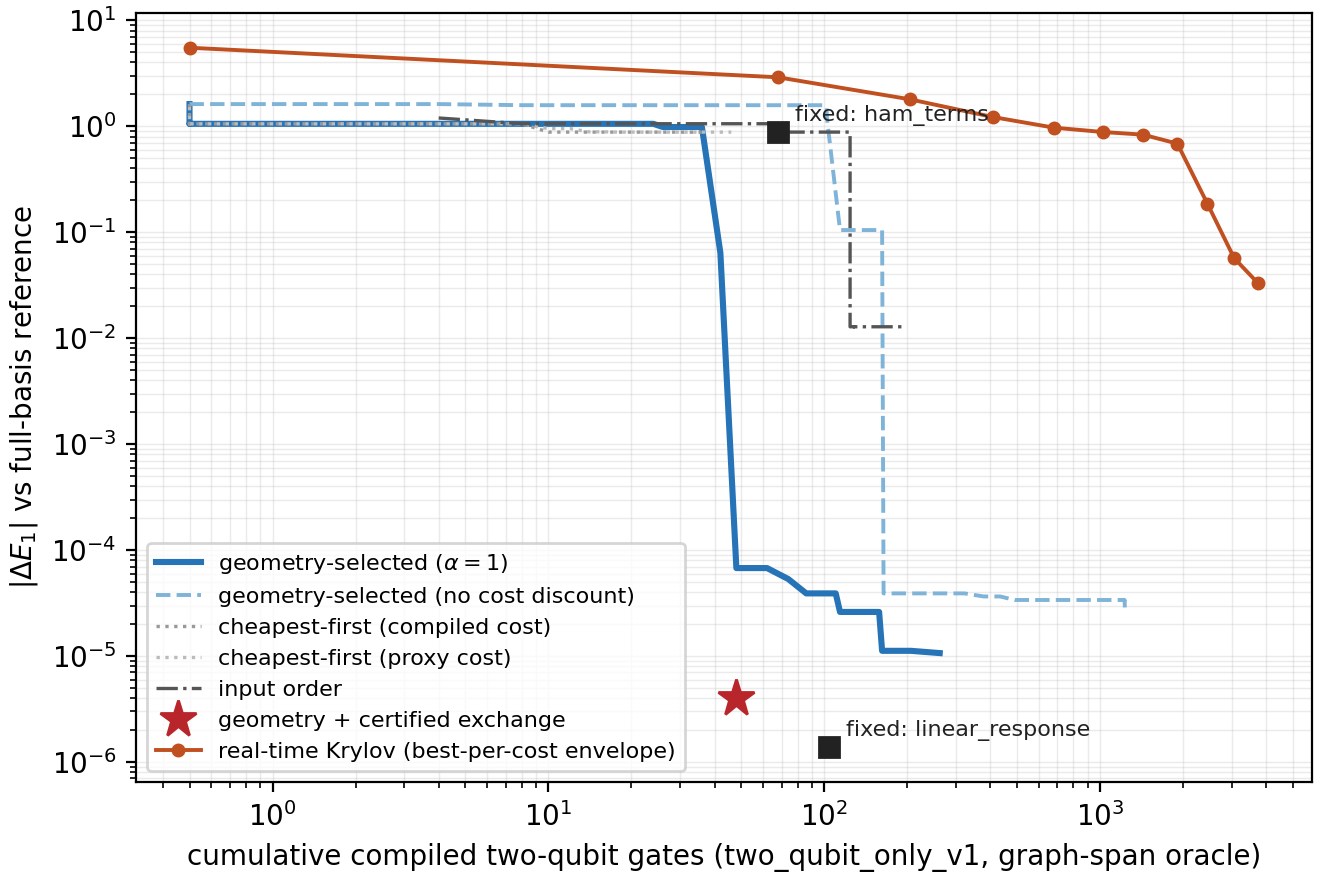
\includegraphics[width=\columnwidth]{generated/paper_iii_frontier_figure.pdf}
\caption{Accuracy--cost frontier at the stored weak-coupling dimer point:
first-excitation error against cumulative compiled two-qubit cost
(\texttt{two\_qubit\_only\_v1}, graph-span oracle, cross-validated against
full transpilation at Spearman $0.9999$).  Cheapest-first orderings never
descend, input order stalls, and the Krylov best-per-cost envelope
(baseline-favoring conventions) remains above $3\times10^{-2}$ at
$70\times$ the cost; the geometry-selected acquisition drops five decades
at ${\sim}40$--$50$ gates, and certified exchange (star) reaches within
$3\times$ of the complete linear-response class's accuracy at under half
its cost.  Regenerated from the committed evidence records by
\texttt{pipelines/reporting/build\_paper\_iii\_frontier\_figure.py}.}
\label{fig:qse_frontier}
\end{figure}

\begin{figure}[t]
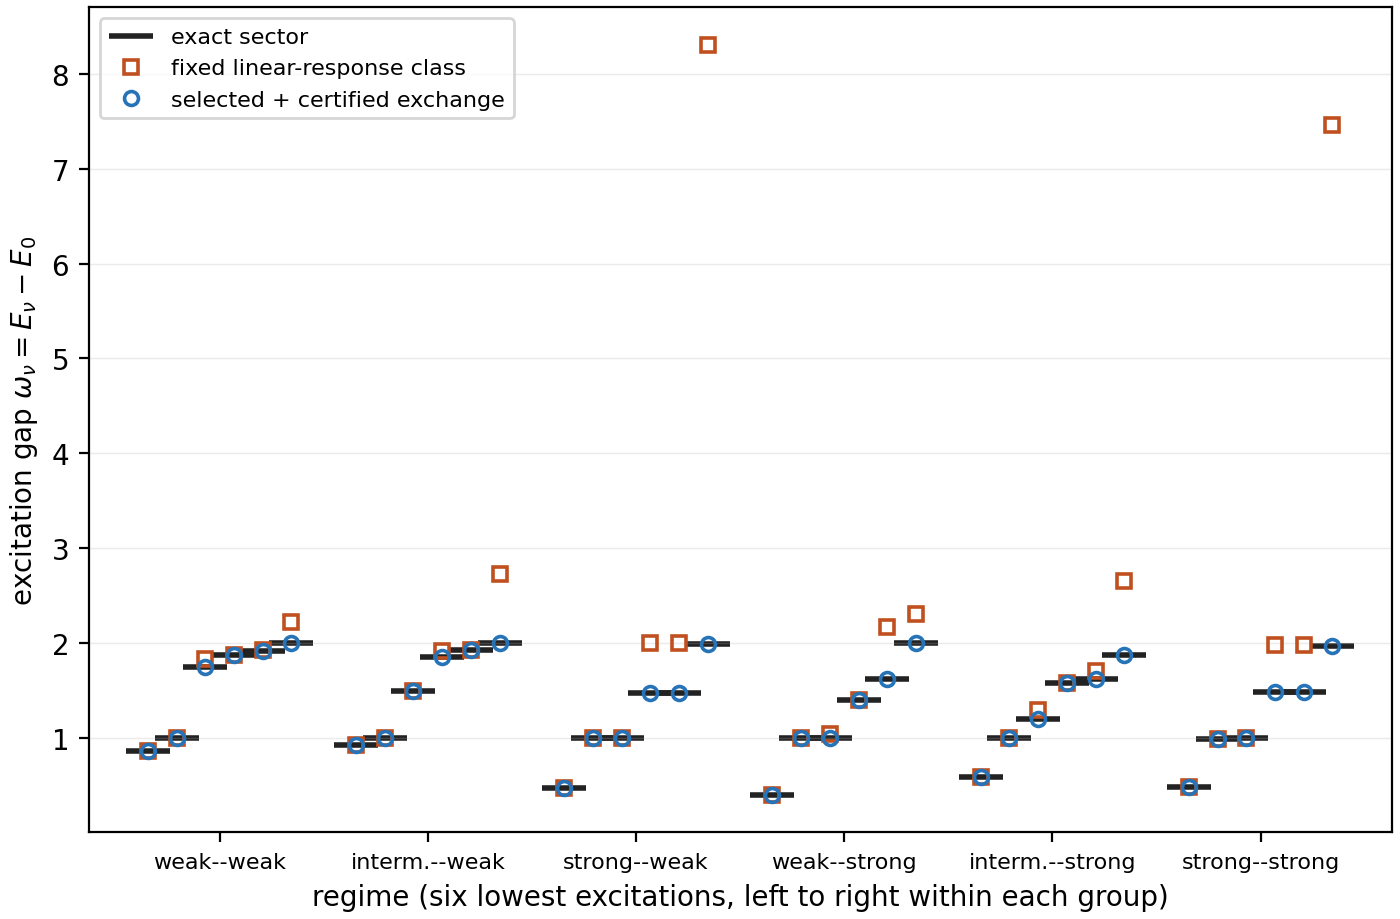
\includegraphics[width=\columnwidth]{generated/paper_iii_gap_figure.pdf}
\caption{Excitation gaps $\omega_\nu=E_\nu-E_0$ for the six lowest excitations of each Paper-I regime (ordered left to right within each group): exact sector-restricted spectrum (bars) against the complete fixed linear-response class (squares) and the geometry-selected support with certified exchange (circles).  The selected support lies on the exact ladder in every regime; the fixed class tracks the low roots in the weak-coupling regimes but places its highest represented root far above the window---$8.3$ against $2.0$ at strong--weak and $7.5$ against $2.0$ at strong--strong---and in the two $u=8$ regimes it misses the lowest excitation entirely, its ladder beginning near $\omega=1$ where the exact spectrum begins near $\omega=0.5$.  Being complete, that class cannot be repaired by additional budget.  The maximum-error column of Table~\ref{tab:qse_multiroot_diag} is the scalar summary of these departures.}
\label{fig:qse_gaps}
\end{figure}

% AUTO-GENERATED by pipelines/reporting/build_paper_iii_tex_fragments.py
% Do not edit by hand; rerun the generator after refreshing evidence.
% source: output/diagnostics/paper_iii_multiroot_sweep_20260818_v1/multiroot_sweep_b60_retained.json

\begin{widetext}
\inlinetablecaption{tab:qse_multiroot_diag}{Statevector-diagnostic multi-root accuracy over the six Paper-I Hubbard--Holstein regimes (lowest six excitations, exact sector-restricted references, budget 60, Ky Fan $R=6$ objective). Cost is compiled two-qubit gate count under the \texttt{two\_qubit\_only\_v1} scalarization.}
\begin{center}
\scriptsize
\begin{ruledtabular}
\begin{tabular*}{\textwidth}{@{\extracolsep{\fill}}llcc@{}}
Regime & Method & compiled 2Q & $\max_{r\le 6}|\Delta E_r|$ \\
\colrule
intermediate\_strong & fixed linear-response class (complete) & 412 & $7.8\times10^{-1}$ \\
intermediate\_strong & geometry-selected ($\alpha=1$, $R=6$) & 14822 & $1.4\times10^{-3}$ \\
intermediate\_strong & geometry + certified exchange & 14156 & $1.4\times10^{-3}$ \\
\colrule
intermediate\_weak & fixed linear-response class (complete) & 104 & $7.3\times10^{-1}$ \\
intermediate\_weak & geometry-selected ($\alpha=1$, $R=6$) & 3504 & $6.9\times10^{-8}$ \\
intermediate\_weak & geometry + certified exchange & 3120 & $4.6\times10^{-8}$ \\
\colrule
strong\_strong\_u8 & fixed linear-response class (complete) & 412 & $5.5\times10^{0}$ \\
strong\_strong\_u8 & geometry-selected ($\alpha=1$, $R=6$) & 9758 & $2.1\times10^{-2}$ \\
strong\_strong\_u8 & geometry + certified exchange & 8516 & $2.7\times10^{-7}$ \\
\colrule
strong\_weak\_u8 & fixed linear-response class (complete) & 104 & $6.3\times10^{0}$ \\
strong\_weak\_u8 & geometry-selected ($\alpha=1$, $R=6$) & 2350 & $5.2\times10^{-1}$ \\
strong\_weak\_u8 & geometry + certified exchange & 1158 & $9.5\times10^{-9}$ \\
\colrule
weak\_strong & fixed linear-response class (complete) & 412 & $5.5\times10^{-1}$ \\
weak\_strong & geometry-selected ($\alpha=1$, $R=6$) & 9006 & $5.4\times10^{-3}$ \\
weak\_strong & geometry + certified exchange & 8960 & $5.4\times10^{-3}$ \\
\colrule
weak\_weak & fixed linear-response class (complete) & 104 & $2.2\times10^{-1}$ \\
weak\_weak & geometry-selected ($\alpha=1$, $R=6$) & 3066 & $4.9\times10^{-7}$ \\
weak\_weak & geometry + certified exchange & 2818 & $3.3\times10^{-7}$ \\
\end{tabular*}
\end{ruledtabular}
\end{center}
\end{widetext}


\begin{widetext}
% AUTO-GENERATED by pipelines/reporting/build_paper_iii_tex_fragments.py
% Do not edit by hand; rerun the generator after refreshing evidence.
% source: output/diagnostics/paper_iii_cost_frontier_arms_20260818_v1/comparator_arms_summary.json
% source: output/diagnostics/paper_iii_cost_frontier_arms_20260818_v1/exchange_maintenance_evidence.json

\inlinetablecaption{tab:qse_comparators_diag}{Statevector-diagnostic cross-family comparison at the weak-coupling dimer point: first-excitation error versus compiled two-qubit cost. The Krylov arm uses a Hamiltonian-residual kick, exact propagation, and Krylov-favoring state-preparation costing.}
\begin{center}
\scriptsize
\begin{ruledtabular}
\begin{tabular}{lcc}
Method & compiled 2Q & $|\Delta E_1|$ \\
\colrule
geometry-selected ($\alpha=1$, $k=20$) & 48 & $6.8\times10^{-5}$ \\
geometry + certified exchange & 48 & $4.0\times10^{-6}$ \\
fixed class: ham\_terms (31 records) & 68 & $8.8\times10^{-1}$ \\
fixed class: linear\_response (18 records) & 104 & $1.4\times10^{-6}$ \\
real-time Krylov (best, $K=11$) & 3740 & $3.3\times10^{-2}$ \\
\end{tabular}
\end{ruledtabular}
\end{center}

\end{widetext}

% AUTO-GENERATED by pipelines/reporting/build_paper_iii_tex_fragments.py
% Do not edit by hand; rerun the generator after refreshing evidence.
% source: output/diagnostics/paper_iii_comparator_matrix_20260819_v1/comparator_matrix.json
% source: output/diagnostics/paper_iii_multiroot_sweep_20260818_v1/multiroot_sweep_epsstop.json
% source: output/diagnostics/paper_iii_peierls_pilot_20260819_v1/peierls_pilot_v4.json

\begin{widetext}
\inlinetablecaption{tab:qse_comparator_matrix}{Cross-family comparator matrix on identical Hamiltonians, sectors, and references: maximum error over the lowest six excitations versus compiled two-qubit cost. The Krylov arm uses a seeded random sector kick (overlapping every target state), exact propagation, best-matching-root scoring, and first-order-Trotter state-preparation costing --- every convention favoring Krylov.}
\begin{center}
\scriptsize
\begin{ruledtabular}
\begin{tabular*}{\textwidth}{@{\extracolsep{\fill}}lccc@{}}
Case & fixed class & real-time Krylov (best) & selected + exchange \\
\colrule
intermediate\_strong & $7.8\times10^{-1}$ @ 412 & $6.8\times10^{-1}$ @ 16632 & $1.2\times10^{-3}$ @ 61364 \\
intermediate\_weak & $7.3\times10^{-1}$ @ 104 & $2.8\times10^{-1}$ @ 3740 & $9.6\times10^{-8}$ @ 2392 \\
peierls\_u8\_weak & $6.8\times10^{0}$ @ 76 & $2.7\times10^{-1}$ @ 6600 & $5.8\times10^{-9}$ @ 214 \\
peierls\_weak\_strong & $5.3\times10^{0}$ @ 76 & $1.8\times10^{-1}$ @ 5500 & $8.3\times10^{-10}$ @ 230 \\
peierls\_weak\_weak & $2.0\times10^{0}$ @ 76 & $1.4\times10^{-1}$ @ 6600 & $1.5\times10^{-10}$ @ 188 \\
strong\_strong\_u8 & $5.5\times10^{0}$ @ 412 & $3.3\times10^{0}$ @ 16632 & $1.6\times10^{-7}$ @ 11270 \\
strong\_weak\_u8 & $6.3\times10^{0}$ @ 104 & $3.2\times10^{-1}$ @ 4488 & $1.4\times10^{-9}$ @ 1452 \\
weak\_strong & $5.5\times10^{-1}$ @ 412 & $7.6\times10^{-1}$ @ 16632 & $5.4\times10^{-3}$ @ 45074 \\
weak\_weak & $2.2\times10^{-1}$ @ 104 & $1.3\times10^{-1}$ @ 4488 & $5.6\times10^{-8}$ @ 5026 \\
\end{tabular*}
\end{ruledtabular}
\end{center}
\end{widetext}


\begin{widetext}
% AUTO-GENERATED by pipelines/reporting/build_paper_iii_tex_fragments.py
% Do not edit by hand; rerun the generator after refreshing evidence.
% source: output/diagnostics/paper_iii_peierls_pilot_20260819_v1/peierls_pilot_v4.json

\inlinetablecaption{tab:qse_peierls_diag}{Statevector-diagnostic generality check on the Peierls--Hubbard dimer (bond-coupled phonon, $n_{\rm ph}=3$): maximum error over the lowest six excitations. The naive fixed class misses the spin-structure directions required by bond coupling.}
\begin{center}
\scriptsize
\begin{ruledtabular}
\begin{tabular}{llcc}
Coupling point & Method & compiled 2Q & $\max_{r\le 6}|\Delta E_r|$ \\
\colrule
peierls\_u8\_weak & fixed linear-response class (complete) & 76 & $6.8\times10^{0}$ \\
peierls\_u8\_weak & geometry-selected ($\alpha=1$, $R=6$) & 254 & $4.2\times10^{-10}$ \\
peierls\_u8\_weak & geometry + certified exchange & 214 & $5.8\times10^{-9}$ \\
\colrule
peierls\_weak\_strong & fixed linear-response class (complete) & 76 & $5.3\times10^{0}$ \\
peierls\_weak\_strong & geometry-selected ($\alpha=1$, $R=6$) & 254 & $3.9\times10^{-10}$ \\
peierls\_weak\_strong & geometry + certified exchange & 230 & $8.3\times10^{-10}$ \\
\colrule
peierls\_weak\_weak & fixed linear-response class (complete) & 76 & $2.0\times10^{0}$ \\
peierls\_weak\_weak & geometry-selected ($\alpha=1$, $R=6$) & 256 & $5.1\times10^{-11}$ \\
peierls\_weak\_weak & geometry + certified exchange & 188 & $1.5\times10^{-10}$ \\
\end{tabular}
\end{ruledtabular}
\end{center}

\end{widetext}

\structlabel{Score-term ablations}
Table~\ref{tab:qse_ablation_matrix} ablates one ingredient of the selection score at a time, at the production stop so that support size is an output.  Three conclusions follow, and none of them is uniform across the regimes.  In the weak-phonon regimes the metric-novelty weight, the residual-capture term, and the cost discount are each individually load bearing: removing any one of them roughly doubles the converged support, multiplies compiled cost by three to four, and prevents convergence altogether, the run instead exhausting its pool at an error one to two orders of magnitude worse.  The metric-novelty result is worth stating explicitly because it differs from the companion ansatz-construction setting, where an analogous novelty term did not improve selection and was removed \cite{PaperI}.  Both settings invert a metric---the Fubini--Study metric of the variational manifold there, the overlap Gram matrix of the nonorthogonal excitation basis here---so the difference is not the presence of a metric but what happens to a redundant admission.  In ansatz construction the angles are re-optimized after every insertion, so a redundant generator is variationally absorbed and costs only depth.  In subspace expansion there is no such re-optimization: the basis is the answer, its retained rank fixes which spectral directions exist at all, and a direction the stabilized pencil cannot represent consumes measurement budget while contributing nothing to the window.  Second, the explicit conditioning penalty is inert: it reproduces the anchor exactly in five of six regimes, because the novelty term already supplies the conditioning control it was meant to add.  Third, the two strong-phonon regimes at $n_{\rm ph}=7$ are pool limited rather than score limited---every arm exhausts the pool within ten percent of the same error---so they carry no ablation signal, and the honest reading of those columns is that no acquisition rule can repair a manifold the record pool does not span.

The exception is instructive.  At strong--strong coupling with $u=8$ the metric-novelty \emph{floor}, as distinct from its weight, is decisive: removing it degrades the maximum error from $1.1\times10^{-7}$ to $4.8\times10^{-1}$, a whole root lost, while the same ablation is benign in every weak-phonon regime.  The floor rejects candidates whose retained-frame-orthogonal component is numerically zero; where the metric is well conditioned such candidates are merely redundant, but in the strongly correlated strong-phonon sector they are the directions whose admission collapses the support.  Weight and floor are therefore not two settings of one knob: the weight ranks useful directions, and the floor excludes unrepresentable ones.


% AUTO-GENERATED by pipelines/reporting/build_paper_iii_tex_fragments.py
% Do not edit by hand; rerun the generator after refreshing evidence.
% source: output/diagnostics/paper_iii_score_ablation_20260819_v1/score_ablation.json

\begin{widetext}
\inlinetablecaption{tab:qse_ablation_matrix}{Selection-score ablations at the production residual stop $\varepsilon=10^{-3}$, so support size $k$ is an output: a redundant term shows as equal accuracy at larger $k$, and a load-bearing term as failure to converge (\texttt{pool\_exhausted}). Entries are $k$ and the maximum error over the lowest six excitations; daggers mark runs that exhausted the pool without meeting the stop.}
\begin{center}
\scriptsize
\begin{ruledtabular}
\begin{tabular*}{\textwidth}{@{\extracolsep{\fill}}lccccc@{}}
Regime & production score (anchor) & no~metric-novelty weight & no~metric-novelty floor & no~residual capture & no~cost discount \\
\colrule
intermediate\_strong & 143$^\dagger$ / $8.9\times10^{-3}$ & 156$^\dagger$ / $8.9\times10^{-3}$ & 176$^\dagger$ / $9.0\times10^{-3}$ & 141$^\dagger$ / $8.8\times10^{-3}$ & 147$^\dagger$ / $8.8\times10^{-3}$ \\
intermediate\_weak & 53 / $1.3\times10^{-7}$ & 104$^\dagger$ / $2.3\times10^{-6}$ & 77 / $1.3\times10^{-7}$ & 113$^\dagger$ / $2.8\times10^{-6}$ & 113$^\dagger$ / $3.7\times10^{-6}$ \\
strong\_strong\_u8 & 84 / $1.7\times10^{-7}$ & 151$^\dagger$ / $6.1\times10^{-6}$ & 138 / $1.4\times10^{-7}$ & 166$^\dagger$ / $5.8\times10^{-6}$ & 86 / $1.3\times10^{-7}$ \\
strong\_weak\_u8 & 88 / $5.5\times10^{-9}$ & 103$^\dagger$ / $3.6\times10^{-9}$ & 106 / $1.2\times10^{-8}$ & 69 / $3.7\times10^{-9}$ & 71 / $9.8\times10^{-9}$ \\
weak\_strong & 144$^\dagger$ / $9.4\times10^{-3}$ & 153$^\dagger$ / $9.9\times10^{-3}$ & 176$^\dagger$ / $1.1\times10^{-2}$ & 143$^\dagger$ / $9.5\times10^{-3}$ & 145$^\dagger$ / $9.5\times10^{-3}$ \\
weak\_weak & 71 / $1.7\times10^{-7}$ & 117$^\dagger$ / $1.4\times10^{-6}$ & 92 / $5.7\times10^{-8}$ & 114$^\dagger$ / $1.1\times10^{-6}$ & 106$^\dagger$ / $1.4\times10^{-6}$ \\
\end{tabular*}
\end{ruledtabular}
\end{center}
\end{widetext}



\subsection{Dynamics results}

\structlabel{Statevector-diagnostic driven dynamics}
Ahead of the production dynamics matrix, Tables~\ref{tab:qse_driven_diag} and~\ref{tab:qse_adaptive_diag} report a completed driven statevector diagnostic at the same Paper-I regime conventions as the static evidence above.  The initial state is the selected first-excitation Ritz root of the residual-stop support; the drive is the staggered-density pulse with the existing envelope conventions ($A=0.2$, $\bar t=4$, $T=8$, 160 midpoint steps), its frequency swept over a grid anchored on QSE-visible transition frequencies out of the initial root (never on exact gaps); frozen propagation uses only the premeasured projected matrices of Eq.~(\ref{eq:frozen_projected_drive}).  This quantity is the McLachlan/Galerkin defect of variational quantum dynamics \cite{Yao2021AVQDS} specialized to a frozen, premeasured pencil, where it is computable from the stored projected and second-moment data without new tangent-space tomography.  In practice its numerator in Eq.~(\ref{eq:frozen_escape}) is most informative before normalization: at a QSE Ritz root the projected residual $(\widehat M-E)y$ vanishes identically, so the entire variance lies outside the retained manifold and the fraction $\rho_{\rm esc}$ is exactly unity at $t=0$ and stays near unity under a weakly switched drive, carrying no magnitude information, whereas the \emph{escape flux} $[\Var_{\Psi(t)}(H(t))-p(t)^\dagger S_\tau^+p(t)]_+^{1/2}$ starts at the static residual---below the selection stop $\varepsilon=10^{-3}$ by construction---and is amplified $40$--$240\times$ by the drive in the four responsive regimes, tracking both the fidelity loss against the exact driven trajectory and the observable errors.  In the two $u=8$ regimes the selected first excitation is the sector spin triplet, which at strong repulsion carries one electron per site and is annihilated by the staggered-density probe: the exact response is numerically zero, the escape flux never leaves its static baseline, and frozen propagation is exact.  The escape diagnostic thus identifies dynamically closed cells without exact references.

\structlabel{Pool-limited escape and the handoff trigger}
Table~\ref{tab:qse_adaptive_diag} reports the adaptive-growth arm at each regime's worst-escape frequency.  Growth admits, whenever the escape flux exceeds $10^{-2}$, the pool record whose manifold-orthogonal component best aligns with the unrepresented drift, rebuilds the retained support, and re-injects the state (re-injection losses $\le10^{-8}$).  The result is a deliberate negative: although admitted records capture up to $\sim$60\% of the instantaneous escape direction at isolated checkpoints (and only a few percent at most others), neither the peak escape flux nor the fidelity improves at the addition cap---the drive continuously regenerates directions outside the span of all remaining pool records applied to the reference, faster than record-level growth can supply them.  Driven escape in these regimes is \emph{pool-limited}.  That adaptive propagation can meet a nonzero residual floor set by a finite operator pool is established \cite{Gomes2023AVQDSGreen}; what the measured-QSE setting adds is that checkpoint record growth fails to convert even substantial instantaneous alignment into sustained fidelity, because the drive regenerates out-of-pool components faster than static records absorb them.  Within the tested architecture and accuracy target---not as a universal statement---escalation to live circuit refinement (Sec.~\ref{sec:excited_dynamics_method}) is therefore the principled response.  Both inputs to that decision, the escape flux and the candidate alignment scan, are premeasurable quantities of the QSE workflow; threshold-plus-pool-scan adaptation itself follows \cite{Yao2021AVQDS}, and what is specific here is that the scan runs entirely on stored record images and routes between record-level enrichment and live propagation.

% AUTO-GENERATED by pipelines/reporting/build_paper_iii_tex_fragments.py
% Do not edit by hand; rerun the generator after refreshing evidence.
% source: output/diagnostics/paper_iii_driven_dynamics_20260819_v1/driven_dynamics.json

\begin{widetext}
\inlinetablecaption{tab:qse_driven_diag}{Statevector-diagnostic frozen-QSE driven propagation on the six Paper-I regimes: initial state is the selected first-excitation Ritz root, driven by the staggered-density gaussian-sinusoid pulse ($A=0.2$, $T=8$, 160 midpoint steps) at the worst frequency of a QSE-anchored sweep. The escape flux $\smash{[\Var_\Psi(H(t))-\|(\widehat M(t)-E)y\|^2]_+^{1/2}}$ is measurement-compatible; its $t{=}0$ value is the static Ritz residual and stays below the selection stop $\varepsilon=10^{-3}$.}
\begin{center}
\scriptsize
\begin{ruledtabular}
\begin{tabular*}{\textwidth}{@{\extracolsep{\fill}}lcccccc@{}}
Regime & $k$ & $\omega^\ast$ & flux $t{=}0$ & max flux & min $|\langle\Psi_{\rm ex}|\Psi\rangle|^2$ & exact response (ptp) \\
\colrule
intermediate\_strong & 143 & 1.423 & $1.4\times10^{-3}$ & $1.4\times10^{-1}$ & 0.9609 & $5.8\times10^{-1}$ \\
intermediate\_weak & 53 & 1.185 & $2.3\times10^{-4}$ & $5.6\times10^{-2}$ & 0.9812 & $5.1\times10^{-1}$ \\
strong\_strong\_u8 & 103 & 0.820 & $3.4\times10^{-4}$ & $3.4\times10^{-4}$ & 1.0000 & $6.5\times10^{-12}$ \\
strong\_weak\_u8 & 59 & 1.074 & $1.1\times10^{-5}$ & $1.1\times10^{-5}$ & 1.0000 & $6.3\times10^{-25}$ \\
weak\_strong & 141 & 1.760 & $4.9\times10^{-3}$ & $2.1\times10^{-1}$ & 0.9454 & $6.6\times10^{-1}$ \\
weak\_weak & 71 & 1.250 & $4.9\times10^{-4}$ & $9.8\times10^{-2}$ & 0.9578 & $8.6\times10^{-1}$ \\
\end{tabular*}
\end{ruledtabular}
\end{center}
\end{widetext}


% AUTO-GENERATED by pipelines/reporting/build_paper_iii_tex_fragments.py
% Do not edit by hand; rerun the generator after refreshing evidence.
% source: output/diagnostics/paper_iii_driven_dynamics_20260819_v1/adaptive_dynamics.json

\inlinetablecaption{tab:qse_adaptive_diag}{Frozen versus adaptive QSE propagation at each regime's worst-escape drive frequency. Adaptive growth admits, when the escape flux exceeds $10^{-2}$, the pool record whose manifold-orthogonal component best aligns with the unrepresented drift, then rebuilds the retained support in place.}
\begin{center}
\scriptsize
\begin{ruledtabular}
\begin{tabular}{lccccc}
Regime & $\omega^\ast$ & min fid.\ (frozen) & min fid.\ (adaptive) & records added & added 2Q \\
\colrule
intermediate\_strong & 1.423 & 0.9609 & 0.9609 & 16 & 4568 \\
intermediate\_weak & 1.185 & 0.9812 & 0.9812 & 16 & 3432 \\
strong\_strong\_u8 & 1.284 & 1.0000 & 1.0000 & 0 & 0 \\
strong\_weak\_u8 & 1.433 & 1.0000 & 1.0000 & 0 & 0 \\
weak\_strong & 1.760 & 0.9454 & 0.9454 & 16 & 40396 \\
weak\_weak & 1.250 & 0.9578 & 0.9578 & 16 & 3386 \\
\end{tabular}
\end{ruledtabular}
\end{center}


\structlabel{Live-circuit handoff validation}
At the stored weak-coupling seed point the full handoff chain was exercised end to end at the worst-escape frequency: the selected first-excitation root of the production support (73 records) was compressed by the compact refit into 32 Pauli words at infidelity $2.1\times10^{-14}$, promoted through the scaffold runtime contract at numerical precision, and propagated with the checkpoint McLachlan route under the identical drive and grid.  Structural adaptation is decisive for the live circuit: against the exact driven trajectory the fixed-support baseline collapses to a minimum fidelity of $0.14$, while adaptive support patching retains $0.64$ (append-only) --- yet no live configuration tested approaches the frozen premeasured pencil at $0.96$, and the deletion-conditioned exchange recipe calibrated for residual-quiet windows degrades to $0.43$: its locally certified deletions accumulate under a drive that never quiets.  The conclusion is symmetric to the pool-limited-escape finding above: at this system size the $73$-record premeasured manifold is a better variational space than a $30$-atom generic operator pool, so the handoff mechanism is validated while its payoff is deferred to settings where the pencil itself is unavailable or too costly --- and the natural repair, seeding the live candidate pool from the selected records' own Pauli children, is left to the production dynamics matrix.

\structlabel{Dynamics results}
The production dynamics Pareto matrix---frozen QSE, adaptive QSE, and QSE-triggered live McLachlan refinement per Hamiltonian class, all starting from the same seed and selected excitation root under the same drive and time grid---and its handoff-ablation companion are deferred to the production data collection; their table designs are retained in the source as the locked contract.  The statevector-diagnostic driven-dynamics evidence above stands in their place for this preprint.

\iffalse
\begin{widetext}
\inlinetablecaption{tab:excited_dyn_claims}{Excited-state driven-dynamics Pareto benchmark by Hamiltonian class and method.}
\begin{center}
\scriptsize
\begin{ruledtabular}
\begin{tabular*}{\textwidth}{@{\extracolsep{\fill}}p{0.10\textwidth}p{0.22\textwidth}cccccccc@{}}
Class & Method & $\overline{|\Delta E_\nu(t)|}$ & $\epsilon_{\obs}^{(2)}$ & $\epsilon_{\rm spec}$ & $\overline{\rho_{\rm esc}}$ & $N_{\twq}^{\rm tot}$ & $D_{\twq}^{\rm tot}$ & $S_{\rm mat}^{\rm proxy}$ & status \\
\colrule
fermionic & frozen QSE & \placeholder{...} & \placeholder{...} & \placeholder{...} & \placeholder{...} & \placeholder{...} & \placeholder{...} & \placeholder{...} & baseline\\
fermionic & adaptive QSE basis & \placeholder{...} & \placeholder{...} & \placeholder{...} & \placeholder{...} & \placeholder{...} & \placeholder{...} & \placeholder{...} & ours\\
fermionic & QSE-triggered live McLachlan & \placeholder{...} & \placeholder{...} & \placeholder{...} & \placeholder{...} & \placeholder{...} & \placeholder{...} & \placeholder{...} & ours\\
\colrule
bosonic & frozen QSE & \placeholder{...} & \placeholder{...} & \placeholder{...} & \placeholder{...} & \placeholder{...} & \placeholder{...} & \placeholder{...} & baseline\\
bosonic & adaptive QSE basis & \placeholder{...} & \placeholder{...} & \placeholder{...} & \placeholder{...} & \placeholder{...} & \placeholder{...} & \placeholder{...} & ours\\
bosonic & QSE-triggered live McLachlan & \placeholder{...} & \placeholder{...} & \placeholder{...} & \placeholder{...} & \placeholder{...} & \placeholder{...} & \placeholder{...} & ours\\
\colrule
fermion--boson & frozen QSE & \placeholder{...} & \placeholder{...} & \placeholder{...} & \placeholder{...} & \placeholder{...} & \placeholder{...} & \placeholder{...} & baseline\\
fermion--boson & adaptive QSE basis & \placeholder{...} & \placeholder{...} & \placeholder{...} & \placeholder{...} & \placeholder{...} & \placeholder{...} & \placeholder{...} & ours\\
fermion--boson & QSE-triggered live McLachlan & \placeholder{...} & \placeholder{...} & \placeholder{...} & \placeholder{...} & \placeholder{...} & \placeholder{...} & \placeholder{...} & ours\\
\end{tabular*}
\end{ruledtabular}
\end{center}
\end{widetext}

\begin{widetext}
\inlinetablecaption{tab:excited_dyn_ablation_matrix}{QSE-to-dynamics handoff ablations. Entries are disabled-minus-full paired changes.}
\begin{center}
\scriptsize
\begin{ruledtabular}
\begin{tabular*}{\textwidth}{@{\extracolsep{\fill}}p{0.23\textwidth}ccccccp{0.20\textwidth}@{}}
Variant & $\Delta\overline{|\Delta E_\nu|}$ & $\Delta\epsilon_{\obs}^{(2)}$ & $\Delta\epsilon_{\rm spec}$ & $\Delta\overline{\rho_{\rm esc}}$ & $\Delta D_{\twq}^{\rm tot}$ & $\Delta S_{\rm mat}^{\rm proxy}$ & interpretation \\
\colrule
frozen QSE only & \placeholder{...} & \placeholder{...} & \placeholder{...} & \placeholder{...} & \placeholder{...} & \placeholder{...} & tests dynamic closure of selected QSE basis\\
no adaptive QSE basis growth & \placeholder{...} & \placeholder{...} & \placeholder{...} & \placeholder{...} & \placeholder{...} & \placeholder{...} & tests residual-driven subspace expansion\\
no escape-triggered live refinement & \placeholder{...} & \placeholder{...} & \placeholder{...} & \placeholder{...} & \placeholder{...} & \placeholder{...} & tests QSE closure trigger\\
live refinement without QSE-root warm start & \placeholder{...} & \placeholder{...} & \placeholder{...} & \placeholder{...} & \placeholder{...} & \placeholder{...} & tests root-refit handoff\\
fixed live-refinement cadence & \placeholder{...} & \placeholder{...} & \placeholder{...} & \placeholder{...} & \placeholder{...} & \placeholder{...} & tests escape-residual gating\\
no QSE root-protection guard & \placeholder{...} & \placeholder{...} & \placeholder{...} & \placeholder{...} & \placeholder{...} & \placeholder{...} & tests collapse into lower roots\\
\end{tabular*}
\end{ruledtabular}
\end{center}
\end{widetext}
\fi

\subsection{Spectral attribution figures}

The main physics figures should use condensed diagnostics, replacing ground-state traces by spectral-window diagnostics:
\begin{equation}
\begin{aligned}
\Acal_g&=\{a\in\Acal:\Omega_a\in\Ecal_g\},
\qquad
\Phi_g=[\ket{\phi_a}]_{a\in\Acal_g},\\
P_{g,\tau}
&=
\Phi_g(\Phi_g^\dagger\Phi_g)_\tau^+\Phi_g^\dagger,
\qquad
x_g^{(\nu)}
=
\bra{\Psi_\nu^{\qse}}P_{g,\tau}\ket{\Psi_\nu^{\qse}},\\
&\hspace{1em}g\in\{f,b,fb,\lf,H,\tau\}.
\end{aligned}
\label{eq:alphabet_attribution}
\end{equation}
Here the class \(g\) is inferred from the admitted operator \(\Omega_a\); it is not an independent label stored in the excitation record.  These attributions are non-exclusive operator-class diagnostics and need not sum to one; an exclusive decomposition would require ordered orthogonalization or a leave-one-class-out attribution rule.
The recommended panels are: excitation energy error versus root index; transition strength recovery versus root index; alphabet attribution versus coupling $g/t$; overlap condition number versus admitted record count; frozen-QSE escape $\rho_{\rm esc}(t)$ versus dynamic observable error; and a Pareto plot of $\epsilon_{\rm spec}$ against $S_{\rm mat}^{\rm proxy}$.

\section{Discussion and conclusion}
\label{sec:discussion}
\label{sec:conclusion}

\structlabel{Mechanistic interpretation}
The selection mechanism is acquisition of operator-generated spectral directions under finite matrix-measurement and circuit budgets.  Probe-transition gain identifies candidate excitations visible to the observables of interest, metric novelty prevents addition of directions already expressible by the current nonorthogonal basis, residual capture measures projected eigen-equation miss, Ritz gain estimates lower-branch spectral improvement, and cost penalties keep the construction from degenerating into a largest-alphabet measurement program.  In dynamics, frozen QSE is efficient when the drive remains inside the selected spectral manifold, adaptive QSE extends the nonorthogonal basis when a small number of extra records closes the residual, and live McLachlan refinement is reserved for roots whose escape diagnostic indicates circuit-level propagation is needed.

\structlabel{Scope, limitations, and future work}
The intended evidence package is a compiled, finite-shot-accounted small-system study with ED used as a diagnostic reference.  Exact spectra and trajectories are reserved for reported root errors, transition strengths, and time-domain observable benchmarks; QSE admission and handoff decisions use measurement-compatible quantities of the prepared seed state and selected excitation basis.  The main unresolved numerical issues are sweep scale, root matching under near-degeneracy, finite-shot generalized-eigenproblem stability, and cutoff stress for phonon-bearing systems.  Hardware validation is useful as a final anchor but should not replace the method's class-wise transfer tests.

\structlabel{Summary}
We presented a geometry-aware QSE acquisition rule and excited-state dynamics route for mixed fermion--boson Hamiltonians.  The method uses an optimized compact ADAPT ansatz as a ground-state seed, ranks excitation records by probe gain, metric novelty, residual capture, Ritz spectral gain, conditioning, and cost, then diagonalizes the selected nonorthogonal manifold to obtain spectra and transition observables.  The primary result is spectral: across six Hubbard--Holstein regimes at two phonon cutoffs, a bond-coupled Peierls--Hubbard family, and a three-site extension, selection with certified exchange resolves the lowest six excitations wherever the record pool spans them, while a complete fixed linear-response class and a real-time Krylov construction fail the same window at comparable or higher compiled two-qubit cost, and at three sites the selected support also outperforms the full pool by avoiding its overlap-conditioning collapse.  The dynamics route is a secondary contribution built on that manifold: it propagates frozen QSE coefficients, monitors an escape diagnostic, and hands selected roots to a live checkpoint McLachlan route through the QSE-root interface, with the escalation criteria computable from premeasured data.  The completed production sweep will give a single accuracy--resource comparison across excitation energies, root fidelities, transition strengths, spectra, driven observables, matrix-measurement cost, overlap conditioning, and compiled quantum resources.

\begin{acknowledgments}
\placeholder{Add funding, compute resources, discussions, and advisor acknowledgments.}
\end{acknowledgments}

\clearpage
\appendix

\section{Benchmark Hamiltonian families}
\label{app:hamiltonian_families}

The benchmark-family definitions use the same Hamiltonian registry and encoding conventions as the ground-state and real-time routes.  This appendix states only the root windows, probe observables, symmetry sectors, and excitation alphabets needed for the excited-state study.  The boson-only controls include Bose--Hubbard-style lattice-boson benchmarks as a standard interacting-boson reference class \cite{Fisher1989BosonLocalization}.

\begin{table*}[t]
\small
\setlength{\tabcolsep}{4pt}
\caption{Excited-state benchmark suite. Values in red are placeholders for the locked repository sweep.}
\label{tab:excited_benchmark_suite}
\begin{ruledtabular}
\begin{tabular*}{\textwidth}{@{\extracolsep{\fill}}p{0.16\textwidth}p{0.25\textwidth}p{0.18\textwidth}p{0.18\textwidth}p{0.17\textwidth}@{}}
Family & Representative parameters & Target roots/probes & Alphabets swept & Held-out stress tests \\
\colrule
Hubbard / extended Hubbard & $L=\placeholder{2--6}$, $U/t=\placeholder{0,2,4,8}$ & density, current, spin & $\Ecal_f,\Ecal_H,\Ecal_\tau$ & strong $U/t$, near-degenerate roots \\
Hubbard--Holstein & $L=\placeholder{2--4}$, $g/t=\placeholder{0--1.5}$, $\omega_0/t=\placeholder{0.5--2}$ & density, $X_i$, $N_{\rm ph}$, $C_{nX}$ & $\Ecal_f,\Ecal_b,\Ecal_{fb},\Ecal_{\lf},\Ecal_H$ & larger cutoff, off-resonant drive \\
Boson-only controls & Bose--Hubbard, harmonic/Kerr chain & displacement, occupation & $\Ecal_b,\Ecal_H$ & high occupation cutoff \\
Spin-boson/Rabi & $\Delta,\omega,g$ sweeps & spin response, displacement & $\Ecal_b,\Ecal_{fb},\Ecal_H$ & ultrastrong coupling \\
Molecular electronic & restricted active spaces & dipole, particle--hole roots & $\Ecal_f,\Ecal_H,\Ecal_\tau$ & stretched bonds \\
Molecular vibronic & small vibronic prototypes & dipole, displacement, vibronic sidebands & $\Ecal_f,\Ecal_b,\Ecal_{fb},\Ecal_{\lf}$ & displaced surfaces / multiple modes \\
\end{tabular*}
\end{ruledtabular}
\end{table*}

\section{Excitation alphabet registry}
\label{app:excitation_alphabets}

The symbolic excitation registry is a deduplicated union of fermionic, bosonic, mixed, Lang--Firsov, Hamiltonian-derived, and tangent-derived records:
\begin{equation}
\Ecal_{\rm registry}
=
\Ecal_f^{(1,2)}
\cup
\Ecal_b^{(1,2)}
\cup
\Ecal_{fb}^{\rm dens}
\cup
\Ecal_{fb}^{\rm bond}
\cup
\Ecal_{\lf}
\cup
\Ecal_H^{(K)}
\cup
\Ecal_\tau .
\label{eq:app_excitation_registry}
\end{equation}
The implementation stores each record with symbolic support, mapped Pauli support, sector label, measurement groups, and compatibility metadata.

\section{QSE measurement and regularization details}
\label{app:qse_measurement_details}

The overlap and Hamiltonian matrices are estimated from grouped Pauli decompositions of
\begin{equation}
\Omega_a^\dagger Q_{\mathfrak s,0}\Omega_b,
\qquad
\Omega_a^\dagger Q_{\mathfrak s,0}H_0Q_{\mathfrak s,0}\Omega_b,
\qquad
\Omega_a^\dagger Q_{\mathfrak s,0}OQ_{\mathfrak s,0}\Omega_b.
\label{eq:app_qse_measurement_operators}
\end{equation}
Finite-shot symmetrization is
\begin{equation}
S\leftarrow\frac12(S+S^\dagger),\qquad
M\leftarrow\frac12(M+M^\dagger),
\label{eq:app_qse_symmetrization}
\end{equation}
followed by metric support truncation and ridge whitening as in Eq.~(\ref{eq:qse_metric_whitening}).  This regularization is part of the scientific protocol, not a numerical afterthought, because excited-state QSE matrix elements are both measurement intensive and sensitive to the retained overlap support \cite{ChoiIzmaylov2023MeasurementQSE,Nakamura2024AdaptiveMeasurementQSE,Kwao2026GEPQSE}.

The generalized eigenvalue equation follows from the Rayleigh quotient in the nonorthogonal QSE basis.  For a retained basis $\{\ket{\phi_a}:a\in\Acal\}$, write a trial state as
\begin{equation}
\ket{\Psi(c)}
=
\sum_{a\in\Acal}c_a\ket{\phi_a}.
\label{eq:app_qse_trial_state}
\end{equation}
Within the nonorthogonal excitation manifold, we retain only coefficient vectors whose Hamiltonian action is self-consistent under the overlap metric.
The overlap matrix $S$ and projected Hamiltonian matrix $M$ play different roles:
\begin{equation}
S_{ab}=\braket{\phi_a}{\phi_b},
\qquad
M_{ab}=\bra{\phi_a}H_0\ket{\phi_b}.
\label{eq:app_qse_sm_def}
\end{equation}
Thus
\begin{equation}
\braket{\Psi(c)}{\Psi(c)}
=c^\dagger S c,
\qquad
\bra{\Psi(c)}H_0\ket{\Psi(c)}
=c^\dagger M c.
\label{eq:app_qse_norm_energy}
\end{equation}
The best approximate eigenstate inside the retained subspace is obtained by minimizing the energy expectation while keeping the trial state normalized.  Equivalently, one may minimize the Rayleigh quotient
\begin{equation}
\varepsilon(c)
=
\frac{c^\dagger M c}{c^\dagger S c},
\label{eq:app_qse_rayleigh}
\end{equation}
or minimize $c^\dagger M c$ subject to the normalization constraint $c^\dagger S c=1$.  Introduce a Lagrange multiplier $\varepsilon$ to enforce the constraint:
\begin{equation}
\mathcal L(c)
=
c^\dagger M c-\varepsilon(c^\dagger S c-1),
\label{eq:app_qse_lagrangian}
\end{equation}
where variations in $c$ are now unconstrained because the constraint has been moved into $\mathcal L$.  Setting the derivative with respect to $c^\dagger$ to zero gives
\begin{equation}
\frac{\partial\mathcal L}{\partial c^\dagger}
=
Mc-\varepsilon Sc
=0,
\label{eq:app_qse_lagrange_stationarity}
\end{equation}
and therefore
\begin{equation}
M c=\varepsilon S c.
\label{eq:app_qse_gep_derivation}
\end{equation}
Therefore $M$ is not a regularized version of $S$: $S$ is the metric of the nonorthogonal basis, while $M$ is the Hamiltonian restricted to that basis.  If the basis were orthonormal, then $S=I$ and Eq.~(\ref{eq:app_qse_gep_derivation}) would reduce to ordinary Hamiltonian diagonalization.

\section{Spectral metrics}
\label{app:spectral_metrics}

For ED-accessible benchmarks, root matching uses Eq.~(\ref{eq:root_matching}).  Static root errors are
\begin{align}
\epsilon_E(\nu)&=|\varepsilon_\nu^{\qse}-E_\nu^{\ed}|,
\nonumber\\
\epsilon_F(\nu)&=1-|\braket{\Psi_\nu^{\ed}}{\Psi_\nu^{\qse}}|^2,
\nonumber\\
\epsilon_T^O(\nu)&=
\left|
|\bra{\Psi_\nu^{\qse}}O\ket{\Psi_0^{\qse}}|^2
-
|\bra{\Psi_\nu^{\ed}}O\ket{\Psi_0^{\ed}}|^2
\right|.
\label{eq:app_root_metrics}
\end{align}
The spectral-window error is
\begin{equation}
\epsilon_{\rm spec}^{O}(\Wcal)
=
\sum_{\nu\in\Wcal}
w_\nu^{O}
\left[
|\Delta\omega_\nu|
+
\lambda_T\epsilon_T^O(\nu)
+
\lambda_F\epsilon_F(\nu)
\right].
\label{eq:app_spectral_error}
\end{equation}

\section{Adaptive QSE during dynamics}
\label{app:adaptive_qse_dynamics}

If frozen-subspace propagation has large escape residual, dynamically enlarge the QSE basis.  At checkpoint $t_k$, score a trial record by
\begin{equation}
\Delta_r^{\qse-\dyn}(t_k)
=
\frac{
|\bra{\bar\phi_r}
[H(t_k)-\expval{H(t_k)}]\ket{\Psi(t_k)}|^2
}{
\braket{\bar\phi_r}{\bar\phi_r}+\lambda_S
}.
\label{eq:app_qse_dyn_gain}
\end{equation}
Let $\mathcal N_{2,k}^{\qse-\dyn}(r)$ denote the same supported metric-residual novelty as Eq.~(\ref{eq:qse_phase2_novelty}), but evaluated against the current dynamic QSE basis at checkpoint $t_k$.
\begin{equation}
\begin{aligned}
\Xi_k^{\qse-\dyn}(r)
&=
\frac{
\Delta_r^{\qse-\dyn}(t_k)
}{
1+K_{\rm meas}(r)+K_{\rm cond}(r)
}
\\
&\quad\times
\mathcal N_{2,k}^{\qse-\dyn}(r).
\end{aligned}
\label{eq:app_adaptive_qse_score}
\end{equation}
Admission occurs when
\begin{equation}
\begin{aligned}
\operatorname{Admit}_{k}^{\qse-\dyn}(r)=1
\iff{}&
\rho_{\rm esc}(t_k)\ge\tau_{\rm esc}
\\
&\wedge\
\Xi_k^{\qse-\dyn}(r)\ge\tau_{\qse}^{\dyn}.
\end{aligned}
\label{eq:app_adaptive_qse_admit}
\end{equation}
The new basis keeps past matrix elements and measures only the new rows/columns needed to continue Eq.~(\ref{eq:frozen_qse_ode}).

\section{QSE-to-McLachlan compression details}
\label{app:qse_to_mclachlan_details}

The root-refit objective in Eq.~(\ref{eq:root_refit}) is optimized with the same canonical optimizer settings as the ground-state ansatz preparation unless a root-specific stress test is being reported.  The final live excited-state circuit is accepted when
\begin{equation}
\begin{aligned}
1-
\left|
\bra{\Psi_\nu^{\qse}}\psi_\nu(\vartheta^\star)
\right|^2
\le\tau_{\rm refit}
\\
\wedge\quad
\left|
\bra{\psi_\nu(\vartheta^\star)}
H_0
\ket{\psi_\nu(\vartheta^\star)}
-\varepsilon_\nu
\right|
\le\tau_E^{\rm refit}.
\end{aligned}
\label{eq:app_refit_accept}
\end{equation}

\section{Live checkpoint-refinement interface}
\label{app:excited_dynamic_controller_details}

The live route is treated as an imported checkpoint-refinement primitive.  The QSE layer supplies the root-refit state, the escape residual, the protected-root set, and the QSE-derived record registry; the live primitive supplies the propagated circuit and any accepted structural edit.  Consequently the dynamics ablations in Sec.~\ref{sec:results} test the QSE handoff: frozen closure, adaptive QSE growth, escape-triggered live refinement, root warm start, and root protection.  Generic McLachlan controller internals are inherited from the live route.

\begin{thebibliography}{99}

\bibitem{PaperI}
J. Strobel and J. Simoni,
``Geometric and resource-aware adaptive ansatz construction for fermion--boson Hamiltonian systems,''
companion paper (Paper I of this series).

\bibitem{PaperII}
J. Strobel and J. Simoni,
``Append--prune McLachlan dynamics,''
companion paper (Paper II of this series).

\bibitem{Hubbard1963}
J. Hubbard,
``Electron correlations in narrow energy bands,''
\emph{Proceedings of the Royal Society A} \textbf{276}, 238--257 (1963).

\bibitem{Holstein1959}
T. Holstein,
``Studies of polaron motion: Part I. The molecular-crystal model,''
\emph{Annals of Physics} \textbf{8}, 325--342 (1959);
``Studies of polaron motion: Part II. The `small' polaron,''
\emph{Annals of Physics} \textbf{8}, 343--389 (1959).

\bibitem{Giustino2017ElectronPhonon}
F. Giustino,
``Electron-phonon interactions from first principles,''
\emph{Reviews of Modern Physics} \textbf{89}, 015003 (2017).

\bibitem{FehskeTrugman2007HolsteinPolaron}
H. Fehske and S. A. Trugman,
``Numerical solution of the Holstein polaron problem,''
in \emph{Polarons in Advanced Materials}, Springer Series in Materials Science Vol. 103, edited by A. S. Alexandrov (Springer, Dordrecht, 2007), pp. 393--461.

\bibitem{HohenadlerLinden2007LangFirsov}
M. Hohenadler and W. von der Linden,
``Lang-Firsov approaches to polaron physics: From variational methods to unbiased quantum Monte Carlo simulations,''
in \emph{Polarons in Advanced Materials}, Springer Series in Materials Science Vol. 103, edited by A. S. Alexandrov (Springer, Dordrecht, 2007), pp. 463--502.

\bibitem{SuSchriefferHeeger1979}
W. P. Su, J. R. Schrieffer, and A. J. Heeger,
``Solitons in polyacetylene,''
\emph{Physical Review Letters} \textbf{42}, 1698--1701 (1979).

\bibitem{WeisseFehske2008}
A. Weisse and H. Fehske,
``Exact diagonalization techniques,''
in \emph{Computational Many-Particle Physics}, Lecture Notes in Physics Vol. 739 (Springer, 2008), pp. 529--544.

\bibitem{TroyerWiese2005}
M. Troyer and U.-J. Wiese,
``Computational complexity and fundamental limitations to fermionic quantum Monte Carlo simulations,''
\emph{Physical Review Letters} \textbf{94}, 170201 (2005).

\bibitem{Schollwoeck2011}
U. Schollw\"ock,
``The density-matrix renormalization group in the age of matrix product states,''
\emph{Annals of Physics} \textbf{326}, 96--192 (2011).

\bibitem{Fisher1989BosonLocalization}
M. P. A. Fisher, P. B. Weichman, G. Grinstein, and D. S. Fisher,
``Boson localization and the superfluid-insulator transition,''
\emph{Physical Review B} \textbf{40}, 546--570 (1989).

\bibitem{Macridin2018ElectronPhonon}
A. Macridin, P. Spentzouris, J. Amundson, and R. Harnik,
``Electron-phonon systems on a universal quantum computer,''
\emph{Physical Review Letters} \textbf{121}, 110504 (2018).

\bibitem{Sawaya2020DLevel}
N. P. D. Sawaya et al.,
``Resource-efficient digital quantum simulation of $d$-level systems for photonic, vibrational, and spin-$s$ Hamiltonians,''
\emph{npj Quantum Information} \textbf{6}, 49 (2020).

\bibitem{SawayaHuh2019VibronicSpectra}
N. P. D. Sawaya and J. Huh,
``Quantum algorithm for calculating molecular vibronic spectra,''
\emph{Journal of Physical Chemistry Letters} \textbf{10}, 3586--3591 (2019).

\bibitem{MacDonell2023VibronicAnalog}
R. J. MacDonell et al.,
``Predicting molecular vibronic spectra using time-domain analog quantum simulation,''
\emph{Chemical Science} \textbf{14}, 9439--9451 (2023).

\bibitem{Navickas2025ChemicalDynamics}
T. Navickas et al.,
``Experimental quantum simulation of chemical dynamics,''
\emph{Journal of the American Chemical Society} \textbf{147}, 23566--23573 (2025).

\bibitem{Li2023VBSElectronPhonon}
W. Li et al.,
``Efficient quantum simulation of electron-phonon systems by variational basis state encoder,''
\emph{Physical Review Research} \textbf{5}, 023046 (2023).

\bibitem{McClean2017QSE}
J. R. McClean, M. E. Kimchi-Schwartz, J. Carter, and W. A. de Jong,
``Hybrid quantum-classical hierarchy for mitigation of decoherence and determination of excited states,''
\emph{Physical Review A} \textbf{95}, 042308 (2017).

\bibitem{Colless2018QSE}
J. I. Colless, V. V. Ramasesh, D. Dahlen, M. S. Blok, M. E. Kimchi-Schwartz, J. R. McClean, J. Carter, W. A. de Jong, and I. Siddiqi,
``Computation of molecular spectra on a quantum processor with an error-resilient algorithm,''
\emph{Physical Review X} \textbf{8}, 011021 (2018).

\bibitem{Higgott2019VQD}
O. Higgott, D. Wang, and S. Brierley,
``Variational quantum computation of excited states,''
\emph{Quantum} \textbf{3}, 156 (2019).

\bibitem{Parrish2019MCVQE}
R. M. Parrish et al.,
``Quantum computation of electronic transitions using a variational quantum eigensolver,''
\emph{Physical Review Letters} \textbf{122}, 230401 (2019).

\bibitem{Jones2019Spectra}
T. Jones, S. Endo, S. McArdle, X. Yuan, and S. C. Benjamin,
``Variational quantum algorithms for discovering Hamiltonian spectra,''
\emph{Physical Review A} \textbf{99}, 062304 (2019).

\bibitem{Nakanishi2019SSVQE}
K. M. Nakanishi, K. Mitarai, and K. Fujii,
``Subspace-search variational quantum eigensolver for excited states,''
\emph{Physical Review Research} \textbf{1}, 033062 (2019).

\bibitem{Ollitrault2020qEOM}
P. J. Ollitrault et al.,
``Quantum equation of motion for computing molecular excitation energies on a noisy quantum processor,''
\emph{Physical Review Research} \textbf{2}, 043140 (2020).

\bibitem{AsthanaKumar2023QScEOM}
A. Asthana et al.,
``Quantum self-consistent equation-of-motion method for computing molecular excitation energies, ionization potentials, and electron affinities on a quantum computer,''
\emph{Chemical Science} \textbf{14}, 2405--2418 (2023).

\bibitem{Grimsley2019ADAPT}
H. R. Grimsley, S. E. Economou, E. Barnes, and N. J. Mayhall,
``An adaptive variational algorithm for exact molecular simulations on a quantum computer,''
\emph{Nature Communications} \textbf{10}, 3007 (2019).

\bibitem{Tang2021QubitADAPT}
H. L. Tang et al.,
``Qubit-ADAPT-VQE: An adaptive algorithm for constructing hardware-efficient ans\"atze on a quantum processor,''
\emph{PRX Quantum} \textbf{2}, 020310 (2021).

\bibitem{Yordanov2021QEB}
Y. S. Yordanov, V. Armaos, C. H. W. Barnes, and D. R. M. Arvidsson-Shukur,
``Qubit-excitation-based adaptive variational quantum eigensolver,''
\emph{Communications Physics} \textbf{4}, 228 (2021).

\bibitem{Anastasiou2024TETRIS}
P. G. Anastasiou, Y. Chen, N. J. Mayhall, E. Barnes, and S. E. Economou,
``TETRIS-ADAPT-VQE: An adaptive algorithm that yields shallower, denser circuit ans\"atze,''
\emph{Physical Review Research} \textbf{6}, 013254 (2024).

\bibitem{Ramoa2025CEO}
M. Ram\^oa et al.,
``Reducing the resources required by ADAPT-VQE using coupled exchange operators and improved subroutines,''
\emph{npj Quantum Information} \textbf{11}, 86 (2025).

\bibitem{Sohail2026GeoADAPT}
M. A. Sohail and T. Koike-Akino,
``Geo-ADAPT-VQE: Quantum information metric-aware circuit optimization for quantum chemistry,''
arXiv:2603.10325 (2026).

\bibitem{McLachlan1964}
A. D. McLachlan,
``A variational solution of the time-dependent Schr\"odinger equation,''
\emph{Molecular Physics} \textbf{8}, 39--44 (1964).

\bibitem{Yuan2019VQS}
X. Yuan, S. Endo, Q. Zhao, Y. Li, and S. C. Benjamin,
``Theory of variational quantum simulation,''
\emph{Quantum} \textbf{3}, 191 (2019).

\bibitem{Barison2021PVQD}
S. Barison, F. Vicentini, and G. Carleo,
``An efficient quantum algorithm for the time evolution of parameterized circuits,''
\emph{Quantum} \textbf{5}, 512 (2021).

\bibitem{Yao2021AVQDS}
Y.-X. Yao, N. Gomes, F. Zhang, C.-Z. Wang, K.-M. Ho, T. Iadecola, and P. P. Orth,
``Adaptive variational quantum dynamics simulations,''
\emph{PRX Quantum} \textbf{2}, 030307 (2021).

\bibitem{Linteau2024APVQD}
D. Linteau, S. Barison, N. H. Lindner, and G. Carleo,
``Adaptive projected variational quantum dynamics,''
\emph{Physical Review Research} \textbf{6}, 023130 (2024).

\bibitem{Zhang2025CompressedAVQD}
F. Zhang, C.-Z. Wang, T. Iadecola, P. P. Orth, and Y.-X. Yao,
``Adaptive variational quantum dynamics simulations with compressed circuits and fewer measurements,''
\emph{Physical Review B} \textbf{111}, 094310 (2025).

\bibitem{ProvostVallee1980}
J. P. Provost and G. Vall\'ee,
``Riemannian structure on manifolds of quantum states,''
\emph{Communications in Mathematical Physics} \textbf{76}, 289--301 (1980).

\bibitem{Stokes2020QNG}
J. Stokes, J. Izaac, N. Killoran, and G. Carleo,
``Quantum natural gradient,''
\emph{Quantum} \textbf{4}, 269 (2020).

\bibitem{Khatri2019QAQC}
S. Khatri, R. LaRose, A. Poremba, L. Cincio, A. T. Sornborger, and P. J. Coles,
``Quantum-assisted quantum compiling,''
\emph{Quantum} \textbf{3}, 140 (2019).

\bibitem{Verteletskyi2020MeasurementGrouping}
V. Verteletskyi, T.-C. Yen, and A. F. Izmaylov,
``Measurement optimization in the variational quantum eigensolver using a minimum clique cover,''
\emph{Journal of Chemical Physics} \textbf{152}, 124114 (2020).

\bibitem{Urbanek2020VQSE}
M. Urbanek, D. Camps, R. Van Beeumen, and W. A. de Jong,
``Chemistry on quantum computers with virtual quantum subspace expansion,''
\emph{Journal of Chemical Theory and Computation} \textbf{16}, 5425--5431 (2020).

\bibitem{Yoshioka2022GQSE}
N. Yoshioka, H. Hakoshima, Y. Matsuzaki, Y. Tokunaga, Y. Suzuki, and S. Endo,
``Generalized quantum subspace expansion,''
\emph{Physical Review Letters} \textbf{129}, 020502 (2022).

\bibitem{CortesGray2022QKSD}
C. L. Cortes and S. K. Gray,
``Quantum Krylov subspace algorithms for ground- and excited-state energy estimation,''
\emph{Physical Review A} \textbf{105}, 022417 (2022).

\bibitem{Motta2024SubspaceReview}
M. Motta et al.,
``Subspace methods for electronic structure simulations on quantum computers,''
\emph{Electronic Structure} \textbf{6}, 013001 (2024).

\bibitem{GolubVanLoan2013MatrixComputations}
G. H. Golub and C. F. Van Loan,
\emph{Matrix Computations}, 4th ed. (Johns Hopkins University Press, Baltimore, 2013).

\bibitem{DavisKahan1970}
C. Davis and W. M. Kahan,
``The rotation of eigenvectors by a perturbation. III,''
\emph{SIAM Journal on Numerical Analysis} \textbf{7}, 1--46 (1970).

\bibitem{Kuhn1955Hungarian}
H. W. Kuhn,
``The Hungarian method for the assignment problem,''
\emph{Naval Research Logistics Quarterly} \textbf{2}, 83--97 (1955).

\bibitem{Epperly2022QSD}
E. N. Epperly, L. Lin, and Y. Nakatsukasa,
``A theory of quantum subspace diagonalization,''
\emph{SIAM Journal on Matrix Analysis and Applications} \textbf{43}, 1263--1290 (2022).

\bibitem{Lee2024SamplingQKSD}
G. Lee, D. Lee, and J. Huh,
``Sampling error analysis in quantum Krylov subspace diagonalization,''
\emph{Quantum} \textbf{8}, 1477 (2024).

\bibitem{Getelina2024HardwareNoiseQSE}
J. C. Getelina, P. Sharma, T. Iadecola, P. P. Orth, and Y.-X. Yao,
``Quantum subspace expansion in the presence of hardware noise,''
\emph{APL Quantum} \textbf{1}, 036127 (2024).

\bibitem{OLeary2025PartitionedQSE}
T. O'Leary, L. W. Anderson, D. Jaksch, and M. Kiffner,
``Partitioned quantum subspace expansion,''
\emph{Quantum} \textbf{9}, 1726 (2025).

\bibitem{Boyd2025ShadowSubspace}
G. Boyd, B. Koczor, and Z. Cai,
``High-dimensional subspace expansion using classical shadows,''
\emph{Physical Review A} \textbf{111}, 022423 (2025).

\bibitem{Kwao2026GEPQSE}
P. F. Kwao, S. P. Sundar, B. Gupt, and A. Asthana,
``Generalized eigenvalue problem in subspace-based excited-state methods for quantum computers,''
\emph{Journal of Chemical Theory and Computation} \textbf{22}, 2892--2903 (2026).

\bibitem{ChoiIzmaylov2023MeasurementQSE}
S. Choi and A. F. Izmaylov,
``Measurement optimization techniques for excited electronic states in near-term quantum computing algorithms,''
\emph{Journal of Chemical Theory and Computation} \textbf{19}, 3184--3193 (2023).

\bibitem{Nakamura2024AdaptiveMeasurementQSE}
Y. Nakamura, Y. Yano, and N. Yoshioka,
``Adaptive measurement strategy for quantum subspace methods,''
\emph{New Journal of Physics} \textbf{26}, 033028 (2024).

\bibitem{Jamet2022GreenQSE}
F. Jamet, A. Agarwal, and I. Rungger,
``Quantum subspace expansion algorithm for Green's functions,''
arXiv:2205.00094 (2022).

\bibitem{Dhawan2024ImagTimeGreen}
D. Dhawan, D. Zgid, and M. Motta,
``Quantum algorithm for imaginary-time Green's functions,''
\emph{Journal of Chemical Theory and Computation} \textbf{20}, 4629--4638 (2024).

\bibitem{Gauthier2024OccupationQSE}
B. Gauthier, P. Rosenberg, A. Foley, and M. Charlebois,
``Occupation-number quantum-subspace-expansion approach to computing the single-particle Green function: An opportunity for noise filtering,''
\emph{Physical Review A} \textbf{110}, 032624 (2024).

\bibitem{Kokcu2024LinearResponse}
E. K\"okc\"u, H. A. Labib, J. K. Freericks, and A. F. Kemper,
``A linear response framework for simulating bosonic and fermionic correlation functions illustrated on quantum computers,''
\emph{Nature Communications} \textbf{15}, 3881 (2024).

\bibitem{Umeano2025KitaevQSE}
C. Umeano, F. Jamet, L. P. Lindoy, I. Rungger, and O. Kyriienko,
``Quantum subspace expansion approach for simulating dynamical response functions of Kitaev spin liquids,''
\emph{Physical Review Materials} \textbf{9}, 034401 (2025).

\bibitem{Backes2023HHDMFT}
S. Backes, Y. Murakami, S. Sakai, and R. Arita,
``Dynamical mean-field theory for the Hubbard-Holstein model on a quantum device,''
\emph{Physical Review B} \textbf{107}, 165155 (2023).

\bibitem{Denner2023HybridEP}
M. M. Denner et al.,
``A hybrid quantum-classical method for electron-phonon systems,''
\emph{Communications Physics} \textbf{6}, 233 (2023).

\bibitem{Dutta2024BosonicChemistry}
R. Dutta et al.,
``Simulating chemistry on bosonic quantum devices,''
\emph{Journal of Chemical Theory and Computation} \textbf{20}, 6426--6441 (2024).

\bibitem{Peng2025BosonHamiltonians}
B. Peng, Y. Su, D. Claudino, K. Kowalski, G. H. Low, and M. Roetteler,
``Quantum simulation of boson-related Hamiltonians: Techniques, effective Hamiltonian construction, and error analysis,''
\emph{Quantum Science and Technology} \textbf{10}, 023002 (2025).

\bibitem{Fischer2025ShadowQSE}
L. E. Fischer, D. Bultrini, I. Tavernelli, and F. Tacchino,
``Large-scale implementation of quantum subspace expansion with classical shadows,''
arXiv:2510.25640 (2025).

\bibitem{Huang2022QDET}
B. Huang, M. Govoni, and G. Galli,
``Simulating the electronic structure of spin defects on quantum computers,''
\emph{PRX Quantum} \textbf{3}, 010339 (2022).

\bibitem{ZhouShang2024EPhQC}
Y. Zhou and H. Shang,
``Exploring electron-phonon coupling using quantum computing methods,''
\emph{Physica Scripta} \textbf{99}, 125105 (2024).

\bibitem{PavosevicFlick2021QEDEOM}
F. Pavo\v{s}evi\'c and J. Flick,
``Polaritonic unitary coupled cluster for quantum computations,''
\emph{Journal of Physical Chemistry Letters} \textbf{12}, 9100--9107 (2021).

\bibitem{Gandon2024NonadiabaticQSE}
A. Gandon, A. Baiardi, P. J. Ollitrault, and I. Tavernelli,
``Non-adiabatic quantum dynamics with fermionic subspace-expansion algorithms on quantum computers,''
\emph{Journal of Chemical Theory and Computation} \textbf{20} (2024); arXiv:2402.15371.

\bibitem{Tkachenko2024QDavidson}
N. V. Tkachenko et al.,
``Quantum Davidson algorithm for excited states,''
\emph{Quantum Science and Technology} \textbf{9}, 035012 (2024).

\bibitem{Zheng2024ADAPTGCIM}
M. Zheng, B. Peng, A. Li, X. Yang, and K. Kowalski,
``Unleashed from constrained optimization: quantum computing for quantum chemistry employing generator coordinate inspired method,''
\emph{npj Quantum Information} \textbf{10} (2024); arXiv:2312.07691.

\bibitem{Zhang2024MEQKSD}
Z. Zhang et al.,
``Measurement-efficient quantum Krylov subspace diagonalisation,''
\emph{Quantum} \textbf{8}, 1438 (2024).

\bibitem{RobledoMoreno2025SQD}
J. Robledo-Moreno et al.,
``Chemistry beyond the scale of exact diagonalization on a quantum-centric supercomputer,''
\emph{Science Advances} \textbf{11} (2025); arXiv:2405.05068.

\bibitem{LiuDeng2026CSQSE}
X. Liu and J. Deng,
``Resource-efficient simulation of molecular ground and excited states based on contextual subspace and quantum subspace expansion,''
\emph{Journal of Chemical Theory and Computation} (2026), DOI 10.1021/acs.jctc.6c00432.

\bibitem{Patra2025PIGenSQD}
S. Patra et al.,
``Physics informed generative machine learning for accelerated quantum-centric supercomputing,''
arXiv:2512.06858 (2025), preprint.

\bibitem{Rammal2026OQKD}
H. Rammal, R. Perrin, S. Ladhari, C. Dutreix, J. Messud, and M. Saubanere,
``Orthogonal quantum Krylov diagonalisation,''
arXiv:2607.09476 (2026), preprint.

\bibitem{WuSimon2000ThickRestart}
K. Wu and H. Simon,
``Thick-restart Lanczos method for large symmetric eigenvalue problems,''
\emph{SIAM Journal on Matrix Analysis and Applications} \textbf{22}, 602--616 (2000).

\bibitem{McCombs2006IVE}
J. R. McCombs and A. Stathopoulos,
``Iterative validation of eigensolvers: a scheme for improving the reliability of Hermitian eigenvalue solvers,''
\emph{SIAM Journal on Scientific Computing} \textbf{28}, 2337--2358 (2006).

\bibitem{Sorensen1992IRA}
D. C. Sorensen,
``Implicit application of polynomial filters in a $k$-step Arnoldi method,''
\emph{SIAM Journal on Matrix Analysis and Applications} \textbf{13}, 357--385 (1992).

\bibitem{Gomes2023AVQDSGreen}
N. Gomes, D. B. Williams-Young, and W. A. de Jong,
``Computing the many-body Green's function with adaptive variational quantum dynamics,''
\emph{Journal of Chemical Theory and Computation} \textbf{19} (2023); arXiv:2302.03093.

\bibitem{Mootz2024AdaptiveGreen}
M. Mootz, T. Iadecola, and Y.-X. Yao,
``Adaptive variational quantum computing approaches for Green's functions and nonlinear susceptibilities,''
\emph{Journal of Chemical Theory and Computation} \textbf{20}, 8689--8710 (2024).

\bibitem{Sambasivam2026TIMESADAPT}
S. Sambasivam et al.,
``TIMES-ADAPT: A quantum algorithm for real-time evolution in low-energy subspaces using fixed-depth circuits,''
arXiv:2603.02305 (2026), preprint.

\bibitem{Berthusen2024MRQDDynamics}
N. Berthusen, F. Alam, and Y. Zhang,
``Multi-reference quantum Davidson algorithm for quantum dynamics,''
arXiv:2406.08675 (2024).

\end{thebibliography}

\end{document}
